\documentclass[letterpaper, 10 pt, journal, twoside]{IEEEtran}
% %------------------------------------------------------------------------------------
%	PACKAGES AND DOCUMENT CONFIGURATIONS
%------------------------------------------------------------------------------------
\usepackage[maxnames=6,firstinits=true,doi=false,url=true,isbn=false]{biblatex}
\addbibresource{IROS.bib}
\usepackage{array}
\usepackage{graphicx}
\usepackage{amsmath}
\usepackage{amssymb}
\usepackage{color}
\usepackage{threeparttable}
\usepackage{balance} %balance columns
\hyphenation{op-tical net-works semi-conduc-tor}
\usepackage{enumitem}
\usepackage{hyperref} % Add  [ocgcolorlinks,pdfusetitle] before hyperref for colored links
% \usepackage{subfig}
\usepackage{subcaption}
\usepackage{dblfloatfix}
\usepackage{booktabs}
\usepackage{authblk}



\newcommand{\TODO}[1]{{\color{red}\textbf{TODO: #1}}}

% \usepackage[english]{babel}
% \usepackage[utf8]{inputenc}
% \usepackage{amsmath}
% \usepackage{graphicx}
% \usepackage[colorinlistoftodos]{todonotes}
% \usepackage[version=3]{mhchem}
% \usepackage{siunitx}
% \usepackage{epstopdf}
% \usepackage{fancyhdr}[18.4]
% \usepackage{placeins}
% \usepackage{lipsum}
% \usepackage{cleveref}
% \usepackage{pdfpages}
% \usepackage{afterpage}
% \usepackage{url}
% \usepackage{booktabs}
% \graphicspath{ {./figs/}}
% \usepackage{array}
% \usepackage{subfig}
% \usepackage{subcaption}
% \usepackage[margin=2cm]{geometry}
% \usepackage{tikz}
% \usepackage{pgfgantt}
% \usetikzlibrary{shapes,arrows}
% \usepackage{verbatim}
% \usepackage{authblk}
% \usepackage{enumitem}
% \usepackage[hang,flushmargin]{footmisc}


% % \usepackage{biblatex}
% \addbibresource{References.bib}




 




\usepackage[maxnames=6,firstinits=true,doi=false,url=true,isbn=false]{biblatex}
% \addbibresource{IROS.bib}
\addbibresource{cav_determinism.bib}
\usepackage{array}
\usepackage{graphicx}
\usepackage{amsmath}
\usepackage{amssymb}
\usepackage{color}
\usepackage{threeparttable}
\usepackage{balance} %balance columns
\hyphenation{op-tical net-works semi-conduc-tor}
\usepackage{enumitem}
\usepackage{hyperref} % Add  [ocgcolorlinks,pdfusetitle] before hyperref for colored links
% \usepackage{subfig}
\usepackage{subcaption}
\usepackage{dblfloatfix}
\usepackage{booktabs}
\usepackage{authblk}
\newcommand{\TODO}[1]{{\color{red}\textbf{TODO: #1}}}
% \pagenumbering{gobble} %suppresses page numbers
\usepackage{balance} %balance columns
%\usepackage{todonotes}
\usepackage[disable]{todonotes}
\usepackage{siunitx}
% \usepackage{draftwatermark}
\usepackage{flushend}

%-------------------------------------------------------------------------------

\begin{document}

% ***************************************************
%  TITLE
% ***************************************************
\title{On Determinism of Game Engines used for Simulation-based Autonomous Vehicle Verification}
% \title{On the Precision of Game Engines used for Simulation-based Autonomous Vehicle Verification}
% \author[1,3]{Abanoub Ghobrial\thanks{$^{1}${\footnotesize \{abanoub.ghobrial, greg.chance, kevin.mcareavey, kerstin.eder\}@bristol.ac.uk}}}
% \author[1,3]{Greg Chance}
% \author[1,3]{Kevin McAreavey}
% \author[2,3]{Severin Lemaignan\thanks{$^{2}${\footnotesize \{severin.lemaignan, tony.pipe\}@brl.ac.uk}}}
% \author[2,3]{Tony Pipe}
% \author[1,3]{Kerstin Eder}
% \affil[1]{Trustworthy Systems Laboratory, University of Bristol, Bristol, UK}
% \affil[2]{University of West of England, Bristol, UK}
% \affil[3]{Bristol Robotics Laboratory, Bristol, UK}

% \author{Abanoub Ghobrial\thanks{$^{1}${\footnotesize \{abanoub.ghobrial, greg.chance, kevin.mcareavey, kerstin.eder\}@bristol.ac.uk}}}
% \author{Greg Chance}
% \author{Kevin McAreavey}
% \author{Severin Lemaignan\thanks{$^{2}${\footnotesize \{severin.lemaignan, tony.pipe\}@brl.ac.uk}}}
% \author{Tony Pipe}

\author{Abanoub Ghobrial, Greg Chance, Kevin McAreavey, Severin Lemaignan, Tony Pipe, Kerstin Eder 
\thanks{{\footnotesize
Manuscript  
received ...;
revised ...;  
accepted.... 
Date of publication ...;
date of current version ....

\textit{Abanoub Ghobrial and Greg Chance contributed equally to this paper and are both corresponding authors.}
%

This research has in part been funded by the ROBOPILOT and CAPRI projects. Both projects are part-funded by the Centre for Connected and Autonomous Vehicles (CCAV), delivered in partnership with Innovate UK under grant numbers 103703 (CAPRI) and 103288 (ROBOPILOT), respectively.
% The Associate Editor for this paper was ....

Abanoub Ghobrial (e-mail: abanoub.ghobrial@bristol.ac.uk), 
Greg Chance (e-mail: greg.chance@bristol.ac.uk), 
Kevin McAreavey (e-mail: kevin.mcareavey@bristol.ac.uk), 
and 
Kerstin Eder (e-mail: kerstin.eder@bristol.ac.uk) 
are with the Trustworthy Systems Lab, Department of Computer Science, University of Bristol, Merchant Ventures Building, Woodland Road,  Bristol, BS8 1UQ, United Kingdom. 

Severin Lemaignan (e-mail: severin.lemaignan@brl.ac.uk)
and
Tony Pipe (e-mail: tony.pipe@brl.ac.uk), 
are with the Bristol Robotics Lab, T Block, University of the West of England,Frenchay, Coldharbour Ln, Bristol, BS34 8QZ, United Kingdom. 

Digital Object Identifier ....
}}}
% \affil{Trustworthy Systems Laboratory, University of Bristol, Bristol, UK}
% \affil{University of West of England, Bristol, UK}
% \affil{Bristol Robotics Laboratory, Bristol, UK}
%
\markboth{IEEE TRANSACTIONS ON INTELLIGENT TRANSPORTATION SYSTEMS VOL. ..., NO. ..., date...}{Ghobrial \MakeLowercase{\textit{et al.}}: On Determinism of Game Engines used for Simulation-based Autonomous Vehicle Verification}
%
\maketitle
%
\begin{abstract}
\noindent 
Game engines are increasingly used as simulation platforms by the autonomous vehicle (AV) community to develop vehicle control systems and test environments. 
%
A key requirement for simulation-based development and verification is determinism, since a deterministic process will always produce the same output given the same initial conditions and event history. 
%
Thus, in a deterministic simulation environment, tests are rendered repeatable and yield simulation results that are trustworthy and straightforward to debug. 
%
However, game engines are seldom deterministic.

This paper first reviews and identifies the potential causes of non-deterministic behaviours in game engines. 
%
A case study using CARLA, an open-source autonomous driving simulation environment powered by Unreal Engine, is then presented to highlight its inherent shortcomings in providing sufficient precision in experimental results. 
%
Different configurations and utilisations of the software and hardware are explored to determine an operational domain where the simulation precision is sufficiently low i.e.\ variance between repeated executions becomes negligible for development and testing work.  

Finally, a method of a general nature is proposed, that can be used to find the domains of permissible variance in game engines simulations for any given system configuration.


% =========================================
% Game engines are increasingly used as simulation platforms by the autonomous vehicle (AV) community to develop vehicle control systems and test environments.
% %
% A key requirement for simulation-based development and verification is determinism.
% %
% Whereby, a deterministic process will always produce the same output given the same initial conditions and event history.
% %
% Thus, making tests repeatable and yielding simulation results that are trustworthy and straightforward to debug.
% %
% However, game engines are seldom deterministic.

% This paper first reviews and identifies the potential causes of non-deterministic behaviours in game engines.
% %
% This is then followed by a case study using CARLA, an open-source autonomous driving simulation environment powered by Unreal Engine, which highlights its inherent shortcomings in providing sufficient precision in experimental results.
% %
% Different configurations and utilisations of the software and hardware are explored to determine an operational domain where the simulation precision is satisfactory low i.e. variance between repeats becomes negligible for development and testing work.  

% Finally, a method of a general nature is proposed, that can be used to find the domains of permissible variance in game engines simulations for any given system configuration.

% =========================================
% Game engines are increasingly used as simulation platforms by the autonomous vehicle (AV) community to develop vehicle control systems and test environments. 
% %
% A deterministic process has no randomness and will always produce the same output with the same initial conditions and event history. 
% %
% Determinism is a key requirement for simulation-based development and verification; it ensures tests are repeatable, so that software bugs can be found and fixed, and simulation results are trustworthy.
% \todo[inline,color=green!40]{GC Alternative: Determinism is a key requirement for simulation-based development and verification; it ensures the simulation is precise and that tests are repeatable, so that software bugs can be found and fixed, and simulation results are trustworthy.}
% %
% % KIE: Ideally, these engines are deterministic, but we've found that they are not. :(
% % These engines must be deterministic for finding and resolving defects (bugs) in software and ensuring auditable and repeatable tests can be executed for verification and validation (V\&V). 
% %
% However, game engines do not need to be deterministic per se. % when used for games. 
% %
% This paper identifies the requirements these engines need to fulfil when used for AV development and testing, and proposes a method to determine the \textit{simulation precision} for specific configurations and utilisation of the software and hardware, respectively. 
% %
% \todo[inline,color=red!40]{old: A case study using CARLA, an open-source simulation environment powered by Unreal Engine, illustrates the proposed method and results from an example scenario indicate the presence of a deterministic operational simulation setup.}
% %
% A case study using CARLA, an open-source autonomous driving simulation environment powered by Unreal Engine has highlighted the shortcomings of using a games engine for simulation based verification. The proposed method and results from an example scenario demonstrate simulation precision to an acceptable tolerance.
% %
% % \textbf{ALTERNATIVE: This empirical investigation using CARLA, an open-source autonomous driving simulation environment powered by Unreal Engine, has highlighted the shortcomings of using a games engine for simulation based verification and we present advice for best working practice.}

\todo[inline,color=green!40]{GC Alternative: A case study using CARLA, an open-source simulation environment powered by Unreal Engine, illustrates the proposed method and results from an example scenario demonstrate simulation precision to an acceptable tolerance. }
\todo[inline,color=yellow!40]{AG Alternative: A case study using CARLA, an open-source autonomous driving simulation environment powered by Unreal Engine (game engine), illustrates the proposed method and results from an example scenario demonstrate simulation precision to an acceptable tolerance. }
\todo[inline]{Review again at end. Potentially give away more on results to motivate the reader to continue.}


% The industry and certification bodies for connected autonomous vehicles is adopting the use of physics and gaming engines to develop, train, verify, validate and certify the software of these autonomous systems in simulation. It is important for these engines to be deterministic in order for one to carry out these different processes. However, such engines are inherently non-deterministic. We propose a method by which one can identify the region where they can operate in these engines and guarantee that the level of non determinism is sufficiently low that it can be assumed to be deterministic. We also implement this method on a case study and show how we identified the region (encompassing computational utilisation and behaviours in simulation) at which one can guarantee performance to be sufficiently deterministic.          
\end{abstract}

\begin{IEEEkeywords}
Autonomous Driving, Autonomous Vehicles, Determinism, Physics Engines,  Verification and Validation (V\&V), Simulation, Testing
\end{IEEEkeywords}
\IEEEpeerreviewmaketitle

% ***************************************************
%  INTRODUCTION
% ***************************************************
\section{Introduction} \label{s:introduction}
% What is verification
% Can't use this again as this is how the AI Test paper starts. -> Avoid self-plagiarism!
%\IEEEPARstart{V}{}erification is the process used to gain confidence in the correctness of a system with respect to its requirements~\cite{bergeron2012writing}. 
%
% Simulation-based verification of autonomous driving functionality is a promising counterpart to costly on-road testing, benefiting from complete control over (virtual) actors and their environment
% , offering a relatively inexpensive means to explore test cases while also
% \IEEEPARstart{S}{}imulation-based techniques can be used to verify autonomous driving functions under development benefiting from full control over the road network and the actors within it. 
\IEEEPARstart{S}{}imulation-based verification of autonomous driving functionality is a promising counterpart to costly on-road testing, that benefits from complete control over (virtual) actors and their environment.
%
Simulated tests aim to provide evidence to developers and regulators of the functional safety of the vehicle or its compliance with commonly agreed upon road conduct~\cite{ViennaConv}, national rules~\cite{codes2015highway} and road traffic laws~\cite{RoadTraffic1988} which form a body of safe and legal driving rules, termed assertions, that must not be violated. 

Design confidence is gained when the autonomous vehicle (AV) can be shown to comply with these rules, e.g.\ through assertion checking during simulation. 
There have been a number of fatalities with AVs, some of which could be attributed to insufficient verification and validation (V\&V), e.g.~\cite{FatalityExample}. Simulation environments offer a means to explore the vast parameter space in a safe and efficient manner~\cite{korosec2019waymo} without the need for millions of miles of costly on-road testing~\cite{kalra2016driving}. In particular, simulations can be biased to increase the frequency at which otherwise rare events occur~\cite{Koopman2018}; this includes testing how the AV reacts to unexpected behaviour of the environment~\cite{RobustnessAutonomy}. 

% The use of game engines for AV testing
Increasingly, the autonomous vehicle community is adopting game engines as simulation platforms to support the development and testing of vehicle control software. 
%
CARLA~\cite{carla_main_website}, for instance, is an open-source simulator for autonomous driving that is implemented in the Unreal Engine~\cite{UE4_main_website}, a real-time 3D creation environment for the gaming and film industry as well as other creative sectors~\cite{CARLA_paper}. 

% Requirements of simulation based verification SBV
State-of-the-art game engines provide a convenient option for simulation-based testing. They offer sufficient realism~\cite{Koopman2018} in the physical domain combined with realistic rendering of scenes, potentially suitable for perception stack testing and visual inspection of accidents or near misses. 
%
Furthermore, they are easy to setup and run with respect to on-road testing and are simple to control and observe, both with respect to the environment the AV operates in as well as the temporal development of actors~\cite{Ulbrich2015}. 
%
%\todo[inline]{These game engines provide a convenient route to testing ego control and perception stack in a realistic environment}
% 
% GC Removing the following para:
%For game engines to be used in simulation-based testing of AVs, they must offer sensors that operate at an accuracy equivalent to those on the AV, e.g.\ video cameras, LIDAR, IR, etc., or interfaces for developers to integrate their own sensor models. CARLA currently offers various basic types of cameras and %ray-case based 
% lidar; extensions are still under development. 
% \todo{GC: what is ray-case? KIE: Not sure. :(}
%
Finally, support for hardware-in-the-loop development or a real-time test-bed for cyber-security testing~\cite{Javaid2013} may also be required. %~\cite{Javaid2013,cyres}
%
% The game engine, in this context, must also comply with the requirements to provide a suitably realistic environment and real-time processing for perception and security analysis.\todo[inline]{next}
%
% Game engines for SBV
Compared to the vehicle dynamics simulators and traffic-level simulators used by manufacturers~\cite{FrameworkAndChallenges}, game engines offer a simulation solution that meets many of the requirements for the development and functional safety testing of AVs in simulation. 
%
However, while game engines are designed primarily for performance to achieve a good user experience, the requirements for AV verification go beyond that and include determinism.

\todo[inline,color=green!40]{GC New below}

\section{Preliminaries}

\subsection{Definitions}

Several definitions are introduced in this section. These are used in the subsequent discussion. Refer to Fig.~\ref{variance_description} throughout this section.
\\

\subsubsection{Determinism}
% What is a deterministic system
Schumann describes determinism as the property of causality given a temporal development of events such that any state is completely determined by prior states~\cite{Schumann2010}. However, in the context of simulation this should be expanded to include not just prior states but also the history of actions taken by all actors. Therefore, a deterministic simulation will always produce the same result given the same history of prior states and actions.
% 
% Herein the term \textit{simulation variance} is used to refer to how simulation traces and outputs vary, when the same stimulus is provided repeatedly to the simulation environment under identical initial conditions. Specifically, we focus on the variance of actor paths within a given scenario. 

A simulation can be thought of as the process of generating or producing experimental data. 
%
In the case of a driving simulator, kinematics will describe future states of actors given the current conditions and actions taken, thereby generating new data. 
%
If a simulation is deterministic, Fig.~\ref{variance_description}~(b), then there will be no variation in the generated output data, i.e. all future states are perfectly reproducible from prior states and actions. 
%
However, if a simulation is non-deterministic, Fig.~\ref{variance_description}~(a), then there will be a variation in the generated output data. \\

\begin{figure}[!t]
    \centering
    \begin{subfigure}{.48\textwidth}
        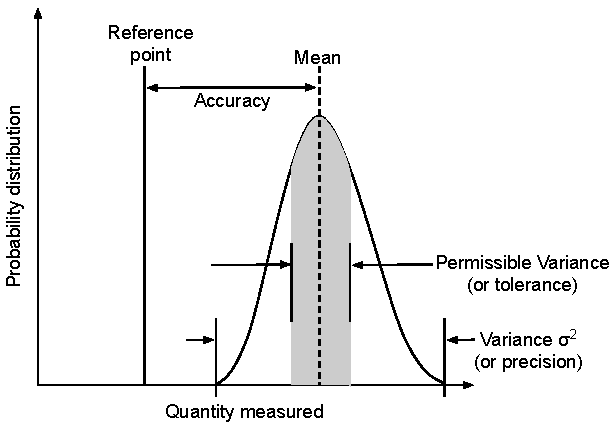
\includegraphics[width=1\textwidth]{Other/Figures/Variance_predicition_tolerance_definition_diagram_a.pdf}
        \caption{Non-deterministic}
        \label{variance_description_a}
    \end{subfigure}

    \begin{subfigure}{.48\textwidth}
        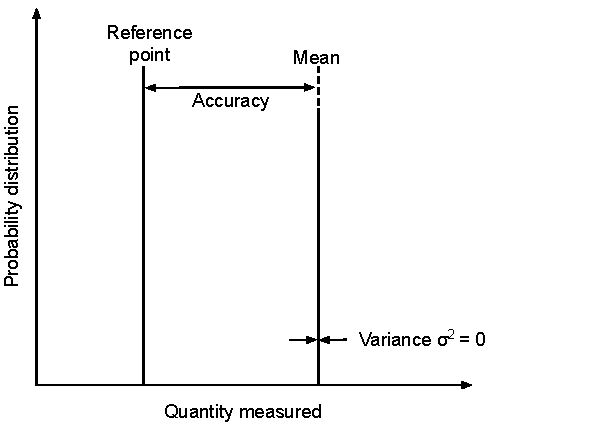
\includegraphics[width=1\textwidth]{Other/Figures/Variance_predicition_tolerance_definition_diagram_b.pdf}
        \caption{Deterministic}
        \label{variance_description_b}
    \end{subfigure}
    \caption{Demonstration of variance, precision, tolerance and determinism}
    \label{variance_description}
\end{figure}


% \subsection{Definitions: Precision, Variance \& Tolerance}
\subsubsection{Variance, Precision \& Tolerance}

We adopt terminology from the mechanical engineering and statistics domains to describe when there is variation in the generated output data~\cite{ADictionaryofMechanicalEngineering}.
%
% \textit{Precision} is therefore defined as the degree to which a simulation can repeatedly generate the same result when executed with the same conditions and actions taken. 
% %
% \textit{Variance} is used here to define the spread (distribution) of the generated output data with respect to the mean value. 
%
% \textit{Variance} (or \textit{precision}) is used here to define the spread (distribution) of the generated output data with respect to the mean value. 
\textit{Variance} is used here to define the spread, or distribution, of the generated output data with respect to the mean value. \textit{Precision} is synonymous with \textit{variance} although inversely related mathematically. 
%
Therefore, variance can indicate the degree to which a simulation can repeatedly generate the same result when executed under the same conditions and actions.
%
\textit{Tolerance} is defined as the permissible limit of the variance, or in short the \textit{permissible variance}. 

% The engineering terms \textit{precision} and \textit{tolerance} suitably describe how the simulation data vary when the same repeated stimulus is provided to the simulation environment under identical initial conditions~\cite{ADictionaryofMechanicalEngineering}. %
%
% As an analogy, the simulator can be thought of as a manufacturing process, producing data and if tasked to repeatedly execute the same process we must ask how \textit{precise} can this process be and what, if any, will the \textit{variance} be? % when comparing the differences between multiple products. 
As an analogy, the simulator can be thought of as a manufacturing process that produces data. To determine the precision of this process, the output must be measured and analysed for differences when the process is repeated. 
%
Those differences describe the spread or variance in the process output. A hard limit on the variance can then be defined, Fig.~\ref{variance_description}~(a), beyond which the output fails to meet the required tolerance, e.g.\ the output is rejected by quality control.
%
% In relation to manufacturing, the precision of any computer based task is casually assumed to be absolute, for example one may question the manufactured precision of a physical component but not the computer assisted drawing that it was made from. 
%but technically this is equivalent to the representation of numbers within it, e.g. 64-bit floating point. %\textbf{[ref]}. %
%
Real manufacturing fails to achieve absolute precision. Hence, there is a need for tolerances to be specified to account for the variance in real-world manufacturing processes. 

If a simulator is deterministic then it will produce results with absolute precision or zero variance, Fig.~\ref{variance_description}~(b), and hence will be within acceptable tolerance by design. If the simulator is non-deterministic then there will be a measurable, non-zero variance in the output data.\\
%

\subsubsection{Accuracy}
Precision and tolerance should not to be confused with \textit{accuracy}, which describes how closely the mean of the generated output of a process aligns to a known standard or reference value. We therefore define accuracy as the difference between the true value, or reference value, and what has been achieved in the data generation process or simulation. 
%
For a driving simulation the reference value 
% , for which accuracy can be measured against, 
may be the real world that the simulation seeks to emulate, where any divergence from this standard is termed the \textit{reality gap}. 
%
In practice full accuracy will often not be achievable due to modelling and associated computational demands of creating and executing exact replica. In most cases, in fact, it is unnecessary and some authors state that `just the right amount of realism' is required to achieve valid simulation results~\cite{Koopman2018}. \\

\subsubsection{Simulation Trace}
A simulation trace is the output log from the simulator consisting of a time series of all actor positions ($x,y,z$) in a 3D environment recorded at regular time intervals. This definition could be extended to include other variables. %, but position is sufficient for this analysis.\\
A set of simulation traces derived from the same input and starting state then forms the experimental data on which variance is calculated for a given simulation run. \\


\subsubsection{Simulation Variance \& Deviation}
If the simulator is non-deterministic then how can the simulation variance be measured? This can be achieved by monitoring the values of any of the recorded output variables that should be consistent from run to run. 
% In this study the actor state was chosen, or more specifically the statistical variance of actor paths within a given scenario using a fixed set of actions. 
For example, actor position variance is a distance-based metric that can be derived from simulation traces. The actor position over time, i.e.\ the actor path, is often used in assertion checking, e.g.\ to determine whether vehicles keep within lanes or whether minimum distances to other vehicles and road users are being maintained. 
% 
Thus, in the case study presented in this paper, the term \textit{simulation variance}, measured in SI unit $m^2$, refers to a measure of actor position variance in the simulation with respect to time, assuming fixed actions. {\color{red} Unclear: Why wrt.\ time, that would then be the actor path, or not?}
%
%\textit{Deviation} (SI unit $m$) is the square root of variance (SI unit $m^2$), which is a more intuitive measure to comprehend when interpreting test results.
%
Case study results are presented using deviation (SI unit $m$), the square root of variance, rather than variance, as this is a more intuitive measure to comprehend when interpreting test results.
%
% more intuitive to comprehend when considering verification tests, e.g. vehicle close-passing. Moreover, the maximum observed value of deviation was chosen over a mean value to ensure sufficient sensitivity.\\
\\

\subsubsection{Scene, Scenario \& Situation}
We adopt the terminology defined for automated driving in~\cite{Ulbrich2015}, where \textit{scene} refers to all static objects including the road network, street furniture, environment conditions and a snapshot of any dynamic elements. Dynamic elements are the elements in a scene whose actions or behaviour may change over time; these are considered actors and may include the AV, or \textit{ego vehicle}, other road vehicles, cyclists, pedestrians and traffic signals. The \textit{scenario} is then defined as a temporal development between several scenes which may be specified by specific parameters. A \textit{situation} is defined as the subjective conditions and determinants for behaviour at a particular point in time.

% \todo[inline]{values - Does this mean stimulus or other parameters? GC - changed to parameters}


% Verification and Determinism 
% Why is determinism important for verification
%For game engines to be useful as a verification tool then they must be deterministic. -> any sim tool must be deterministic, not just game engines ;)
% KE Text
\todo[inline,color=red!40]{old: Determinism is a key prerequisite for simulation during AV development and testing. A deterministic simulation environment guarantees that tests are repeatable. Thus, coverage results are stable and, when a test fails, debugging can rely on the test producing the same trace and outcome when repeated. This ensures that software bugs can be found and fixed efficiently, and that simulation results are trustworthy.  }
%

\subsection{When is Determinism needed?}
Determinism is a key requirement for simulation during AV development and testing. A deterministic simulation environment guarantees that tests are repeatable, i.e.\ repeated runs of a test, given the same initial conditions and event history, produce the same output data.
%
Thus, a deterministic simulator has zero \textit{variance}. 

A simulator with non-zero variance can no longer be considered deterministic. 
%
Non-deterministic simulators may be sufficient for certain applications as long as their variance is permissible, i.e.\ \textit{within tolerance}. 
%
Therefore, \textit{tolerance} is the acceptable degree of variability between repeated simulations. When the simulation output is within tolerance, coverage results are stable and, when a test fails, debugging can rely on the test producing the same trace and outcome when repeated. 
%
This ensures that software bugs can be found and fixed efficiently, and that simulation results are trustworthy.

% GC Text
\todo[inline,color=green!40]{GC Alternative: Determinism is a key prerequisite for simulation during AV development and testing. A deterministic simulation environment guarantees that tests are repeatable. In conventional engineering terms a deterministic simulator can be considered to have zero \textit{tolerance}. If the tolerance is non-zero it can no longer be considered deterministic but this may be sufficient for certain applications as long as it is \textit{within tolerance}. Therefore, \textit{tolerance} is the acceptable degree of variability between repeated execution outputs. When the simulation output is within tolerance, coverage results are stable and, when a test fails, debugging can rely on the test producing the same trace and outcome when repeated. This ensures that software bugs can be found and fixed efficiently, and that simulation results are trustworthy.}

% This is not to be confused with \textit{accuracy} that describes the extent to which the simulation complies to a known standard, which could be considered a level of realism that faithfully describes the real world. The \textit{precision} of the process is the ability of the simulation to repeat the same execution and find no, or a \textit{tolerable}, difference in the outcome. \textit{Tolerance} is the acceptable degree of variability between repeated execution outputs. When the simulation output is within tolerance, coverage results are stable and, when a test fails, debugging can rely on the test producing the same trace and outcome when repeated. This ensures that software bugs can be found and fixed efficiently, and that simulation results are trustworthy. }
%
%Any software defects that are detected but not repeatable at a later time or by another party does not allow for suitable resolution. Furthermore, defects not found on the verification testing system may arise on a deployed system with a different hardware architecture resulting in untested and potentially unsafe behaviour. 
%When considering the development of autonomous vehicles, untested code could lead to dangerous behaviours not being identified and fatal road accidents may occur.
%

If the simulation is non-deterministic, e.g.\ 
% KIE No, whether the variance is or is not permissible is not what matters for non-det, it should be zero!
%e.g. it has a non-permissible variance in,
it has a non-zero variance in, for example, actor positions, then this may, in the best case, lead to intermittent assertion failures, making it difficult to re-produce, understand and remove bugs and rendering verification results unstable. In the worst case, however, bugs that could have been identified in simulation remain undetected, leading to false confidence in the safety of the AV's control software. 
%

% \todo[inline]{GC Edit: If the simulation is non-deterministic, it lacks the appropriate precision for this application and the error between output traces exceeds the acceptable tolerance however, variance in actor positions, for instance, may lead to assessment errors, making it difficult to understand and remove bugs. In the worst case, bugs that could have been identified in simulation remain undetected, resulting in false confidence in the safety of the AV's control software.}

% Challenges of SBV
When used for gaming, game engines do not need to be deterministic nor do they have any requirements on the limits of permissible variance; there are no safety implications from non-determinism in this domain, nor is finding and fixing all the bugs % related to non-determinism 
a high priority for games developers. It could even be argued that simulation variance is a feature that enhances gaming and improves the user experience. However, the situation is very different for AV development and testing. Thus, our main research questions are:
%
\todo[inline,color=red!40]{old: How can one assess the extent to which a simulation environment is deterministic?  }
%
{\em How can one assess whether a simulation environment is deterministic?} and 
{\em How can one determine and control the simulation variance?}
\todo[inline,color=green!40]{GC Alternative: How can one assess the extent to which a simulation environment is deterministic or has a permissible tolerance?} 

% In pursuit of an answer to this question we
In this paper we investigate non-determinism and how it affects simulation results on the example of CARLA, an open-source autonomous driving simulation environment based on the Unreal game engine.
%
In our case study, scenarios between pedestrian and vehicle actors are investigated to determine the actor position variance in the simulation output for repeated simulation runs. 
% KIE: This is covered in the next sentence:
% to identify conditions that result in non-determinism based on actor position variance in the simulation output.
%
\todo[inline,color=red!40]{old: By limiting the level of system utilisation to less than 75\% and terminating scenarios once a collision has been detected, a deterministic operational simulation setup could be identified. }
%
% By analysing actor position variance 
We find that the CARLA simulator is non-deterministic under certain conditions. {\color{red} Say what the observed variance range is, and what we consider permissible for this study.}
% However, by limiting the level of system utilisation to less than 75\% and terminating scenarios once a collision has been detected, a permissible level of simulation variance was observed.
%
CARLA exhibits a permissible level of variance when system utilisation is restricted to 75\% or less and the simulation is terminated once a vehicle collision has been detected. {\color{red} Why ``vehicle'' collision and not just ``collision''?}
%
\todo[inline,color=green!40]{GC Alternative: By analysing actor position variance we find that the Carla simulator is non-deterministic under certain conditions. 
However, by limiting the level of system utilisation to less than 75\% and terminating scenarios once a collision has been detected, a permissible level of simulation variance was observed.}

The insights gained from this case study motivated the development of a general step-by-step method for AV developers and verification engineers to determine the simulation variance for a given simulation environment. 
%
\todo[inline,color=red!40]{old: Knowing the simulation variance will help them assess the impact that using a game engine for AV simulation may have. In particular, they can gain a better understanding of how potentially existing non-determinism affects repeatability and reliability of the simulation results.  }
%
Knowing the simulation variance will help assess the suitability of a game engine for AV simulation.
%impact that using a game engine for AV simulation may have.
% on verification tasks. 
In particular, this can give a better understanding of the effects of non-determinism and to what extent simulation precision may impact on verification results.
%
\todo[inline,color=green!40]{GC Alternative: Knowing the simulation variance will help verification engineers assess the impact that using a game engine for AV simulation may have. In particular, this can give a better understanding of how potentially existing non-determinism affects simulation precision and any verification results that are interpreted from this. }
%
% \todo[inline]{review and potentially summarize results from case study GC - added see below.}
%We present a case study to illustrate the use of this method. The study highlights the effects of non-determinism of a game engine on simulation results. Scenarios between pedestrian and vehicle actors are used to identify conditions that result in high simulation variance.
%
%By limiting the level of system utilisation to less than 75\% and terminating scenarios once a collision has been detected, a deterministic operational domain could be identified.
%

This paper is structured as follows.
%
Section~\ref{s:background} briefly introduces how game engines work before investigating in Section~\ref{s:nondeterminisimSources} the potential sources of non-determinism in game engines.
%
Our case study of simulation variance for a number of scenarios involving pedestrian and vehicle settings using CARLA is presented in Section~\ref{s:case-study}.
%
Section~\ref{s:methodology} presents the step-by-step method to assess the suitability of a simulation system for AV verification in general. 
%
We conclude in Section~\ref{s:conclusion} and give an outlook on future work.\todo{review at end}


% \noindent \IEEEPARstart{T}{}he evolution and inevitable implementation of connected and autonomous vehicles (AVs) on roads is a delicate if not utterly fascinating subject. Such systems operate in environments marked by inaccessibility, unexpected weather conditions, or unpredictable behavior by surrounding humans\cite{RobustnessAutonomy}. 

% Public safety is clearly a prime concern for putting autonomous vehicles into play, which means the meticulous and thorough process of developing, training, verifying, validating and certifying the artificial intelligence (AI) and software of the vehicle is a task to be handled with care. 

% It requires lots of flexibility and room to iterate to ensure the algorithms are given the sharpest understanding for maximum performance as well as to ensure that they are hazard-free in order for them to be deployed\cite{AirsimUnrealArticle}.\\\\

% \noindent There has been a number of catastrophic fatalities with self-driving vehicles due to lack of verification and validation (V\&V) of software e.g.\cite{FatalityExample}.

% As such, there appears the need for finding ways to V\&V the safety of such software, ranging from AI development to cyber-security, while maintaining minimal risks in testing.\\\\

% ======================
% This is all from "FrameworkAndChallenges" without using quotes 
% \noindent Existing vehicle manufacturers use vehicle dynamic simulators to model the physics of each component in a system. Similarly, the use of simulation for traffic modelling is well established. Despite these proven simulation tools, non of them provide all of the required functionalities together to fully simulate AVs\cite{FrameworkAndChallenges}.\\\\

% While traffic-level simulators can model road layouts, they do not require as much realism or detail as AVs require. On the other side, vehicle dynamics simulators include some of the high fidelity physics functionalities needed for AV testing, but they only consider the vehicle itself and perhaps the road surface and gradient; they do not model any of the road layout, signs, traffic/street lights, other street furniture or surrounding infrastructure. 
% Most critically, neither types of simulators model sensors such as cameras, lidars or radars\cite{FrameworkAndChallenges}.\\\\ 
% Consequently, one of the major routes AVs developers are moving towards is using physics engines, these are often games engine development frameworks, since they tick all of the boxes needed to fully simulate AVs \cite{FrameworkAndChallenges}.  
% ======================

% Robopilot, Capri, CARLA, Apollo, Airsim, Udacity etc. are all examples of driving simulator projects that use physics engines to support development, training, and validation of autonomous driving systems software\cite{ListOfSimulators}. \\\\
% Test-retest reliability, is a key factor in V\&V of software. Tests need to be repeatable in order for one to eliminate bugs. 
% In other words physics engines has to be deterministic, or the level of non-determinism of the engine should be low and clearly defined, for them to be used in the context of V\&V of AV software.\\\\
% \TODO{Remove this paragraph?} Determinism of game (physics) engines has not attracted much attention by engines' developers nor researchers. This previously was not important since in gaming, determinism is not critical. 
% Performance, on the other hand, is a subject of more interest in that field, where developers want games to work on all platforms and still be fast to provide a positive user experience. 
% On the contrary, determinism becomes vital and performance not when such engines are used in autonomous vehicles' AI development and testing. \\\\

% This paper aims to investigate how deterministic physics engines are for usage in V\&V for AV simulations; and will cover the list of following points:
% \begin{itemize}[leftmargin=*]
%     \item Necessary background on game engines used in AV simulations.
%     \item Review of sources of non-determinism in such engines.
%     \item Provide a method of how the level of non-determinism can be investigated and defined.
%     \item A case study showing the implementation of this methodology in an engine widely used in AVs simulations (Unreal Engine).
% \end{itemize}
 
% ***************************************************
%  BACKGROUND
% ***************************************************
\section{Background} \label{s:background}

There are numerous game engines with their associated development environments which could be considered suitable for AV development, e.g.\ Unreal Engine~\cite{UE4_main_website}, Unity~\cite{Unity_main_website}, CryEngine~\cite{CryEngine_main_website}. Specific autonomous driving research tools have been created to abstract and simplify the development environment, some of which are based on existing game engines, e.g.\ CARLA~\cite{carla_main_website}, AirSim~\cite{AirSim_main_website}, Apollo~\cite{Apollo_main_website}, and some have been developed for cloud-based simulation, e.g.\ Nvidia Drive Constellation~\cite{nvidia_constellation}.
% \footnote{\url{https://www.nvidia.com/en-gb/self-driving-cars/drive-constellation/}}.

Investigating the determinism of game engines has not attracted much research interest since performance is more critical for game developers than accurate and repeatable execution.  %However, when these engines are used for AV development then deterministic behaviour is required. 
%
Ensuring software operates deterministically is a non-trivial task.  Catching intermittent failures, or flaky tests~\cite{intermittently-failing-tests}, in a test suite that cannot be replayed makes the debugging process equally difficult~\cite{acm-q-rr-interview}.
%
\todo[inline]{GC line added to introduction. We need a paragraph on how hard it can be to make a computation fully determinisitc, referring to the ACM queue interview with the {\tt rr} developers~\cite{acm-q-rr-interview}. Not sure whether this should be in the introduction, HERE, or in a related work section or in the discussion/conclusion. But it is important that we demonstrate knowledge of others working on this in other areas. {\tt rr} is somewhat closely related as they need determinism for debugging, and we need it for that purpose too, although we also need verification results to be stable.}
%
\todo[inline,color=green!40]{GC Addition: Ensuring software operates deterministically is a non-trivial task and catching intermittent failures in a test suite that cannot be replayed makes the debugging process equally difficult~\cite{acm-q-rr-interview}. }
%
This section gives an overview of the internal structure of a game engine and what sources or settings in the engine may affect \textit{simulation variance}.
%
% \noindent This section overviews important information and concepts in physics engines, which are relevant to their usage in AV simulations. Particularly, on how physics engines operate and the sources of non-determinism in these engines necessary to understand the contribution of this paper.

% ======= Overview of a Game Loop
% \subsection{Game Engine Overview} \label{GameLoopSection}

Central to a game engine are the main game logic, the artificial intelligence (AI) component, the audio engine, and the physics and rendering engines. For AV simulation, we focus on the latter two.
%
The game loop is responsible for the interaction between the physics and rendering engines. Fig.~\ref{GameEngineLoopDiagram} depicts a simplified representation of the process flow in a game engine loop, where  initialisation, game logic and decommissioning have been removed~\cite{unity_event_execution}.
% \footnote{\url{https://docs.unity3d.com/Manual/ExecutionOrder.html}}. 
A game loop is broken up into three distinct phases: processing the inputs, updating the game world (Physics Engine), and generating outputs (Rendering)~\cite{GameEngineArchBook}.

\begin{figure}[h]
\centering
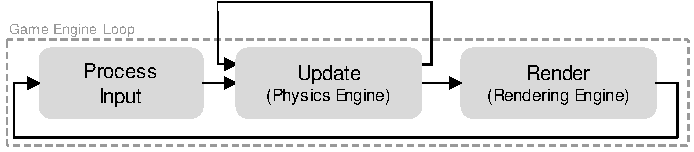
\includegraphics[width=0.5\textwidth]{Other/Figures/GameEngineLoopv2.pdf}
\caption{Game engine loop block diagram~\cite{GameProgPatternsBook}.}
\label{GameEngineLoopDiagram}
\end{figure}

% \todo[inline]{AG: remove the clock symbol, possibly remove the ticks chart as this is confusing given they are not ticks but event markers}

% The first part of the game loop is to process the user inputs which may take the form of user keyed inputs or, in the case of AV development, the response of the AV to the current state of its environment. For example, the throttle and steering angle from the controller of an AV. The update stage interprets the input from all dynamic actors in the scene, performs any necessary physics calculations and updates the actor states. The rendering engine then takes the updated actor states and renders the scene~\cite{GameProgPatternsBook}. 

% \todo[inline]{Fig 1: update rates of which clock? GC-is a clock confusing as it does not run on a 'clock' in computer science terms, rather it is a timer which is used as reference to compare to a 'wall clock'}

% \todo[inline]{Should there not also be a clock in the overall loop? GC-yes the wall clock but it may get confusing as that is a real clock and the game loop clock is a timer?}

% \todo[inline]{Greg to look up Unity wrt concurrently running processes and clocks. Unity page on multi-threading \footnote{\url{https://docs.unity3d.com/Manual/JobSystemMultithreading.html}} and a plugin for multi-thread management \footnote{\url{https://forum.unity.com/threads/task-for-unity-scripting-threading.462971/?_ga=2.228561631.331624405.1587372521-1435703724.1587372521}}} 

% 
% It is necessary to have an understanding of how the game loop operates in order to understand potential sources of non-determinism that are discussed below. 

% \todo[inline]{We should agree if the 'game clock' really is a clock or just times the computation for each game loop.}

% \todo[inline]{For AG: We use the phase 'game clock tick'- where did the come from as I think it is misleading.}

% As the game progresses, the game loop runs continuously according to the game clock. \todo[inline]{introduce the different clocks and what they govern, real world, game, physics and render}
%
% At the beginning of each game clock tick, the lag\todo[inline]{first explain where the lag comes from} between the game clock and the real world is updated based on how much real time has passed. This measures how far the game's clock is behind compared to the real world. 

The game loop cycle starts with initialising the scene and actors. Input events from the User or AI are then processed followed by a physics cycle which may repeat more than once per rendered frame if the physics time step, $dt$, is less than the render update rate. This is illustrated by the loop in the physics update in Fig.~\ref{GameEngineLoopDiagram}. The render update will process frames as fast as the computational processing will allow up to the maximum monitor refresh rate~\cite{unity_framerates}.
% \footnote{\url{https://blogs.unity3d.com/2019/06/03/precise-framerates-in-unity/}}. 
When the frame is rendered the game loop cycle returns to processing inputs. An intuitive and  more detailed description of the interplay between the physics and render cycles is given in~\cite{JohnAustinUnity}.

% \todo[inline]{GC maybe replace this entire section with a briefer account: The game loop cycle starts with initialising the scene and actors. Input events from the User or AI are then processed followed by a physics cycle which may repeat more than once per rendered frame if the physics time step, $dt$, is less than the render update rate. The render update will process frames as fast as the computational processing will allow up to the maximum monitor refresh rate\footnote{\url{https://blogs.unity3d.com/2019/06/03/precise-framerates-in-unity/}}. When the frame is rendered the game loop cycle returns to processing inputs.}
%
% Then the user inputs are processed. There is then an inner loop to update the physics processes (clock symbol in Fig.~\ref{GameEngineLoopDiagram}), incrementing at a delta time step, $dt$, until the game clock is equal to the real world. Rendering occurs once the game clock has caught up with the real world clock. The process then repeats.

The physics engine operates according to a time step, $dt$. %, because it makes everything simpler and more stable for physics and AI.
The shorter this time step is, the smoother the interpretation of the physical dynamics will be. %processing time it takes to catch up to game clock. % and the more deterministic the engine becomes and vice versa, as will be explained in section \ref{s:nondeterminisimSources}. 
%
% Fixing the physics time step to a constant $dt$ results in simpler and more stable physics simulation and AI. 
%
To use a fixed physics time step, the user's display refresh rate needs to be known in advance. This requires an update loop to take less than one render tick (one frame of real world time). Given the range of different hardware capabilities, a variable delta time is often implemented for game playing, taking the previous frame time as the next $dt$. However, variable $dt$ can lead to different outcomes in repeated tests and in some cases unrealistic physical representations~\cite{gaffer}. 
%
Semi-fixed or limited frame rates ensure $dt$ does not exceed some user-defined limit to meet a minimum standard of physical representation but allow computational headroom for slower hardware. Some engines provide sub-stepping which processes multiple physics calculations per frame at a greater CPU cost, e.g.\ Unreal Engine~\cite{UE4_substepping}. 
%
If the engine tries to render between physics updates, \textit{residual lag} can occur, which may result in frames arriving with a delay to the simulated physics.
%
Thus, extrapolation between frames may need to be performed to smooth transition between scenes. 
%
Note that both residual lag and extrapolation could affect perception stack testing.
% This is depicted in the lower part of Fig.~\ref{GameEngineLoopDiagram}. 
% \cite{GameEngineArchBook}\cite{GameProgPatternsBook}\todo[inline]{Should this still be cited? GC-No, it is cited elsewhere.}
%
% \todo[inline]{Why is this part of the figure? It would be clearer if it was in a separate figure that shows all the clocks involved and how they interact - depend on each other. GC-suggest we remove as the ticks are not relevant to the main argument or discussion.}
%
% Ideally the time step should be as short as possible, so that the simulation returns better accuracy of complex physical processes. %runs with high fidelity on fast machines. 
In exceptional cases, where computational resources are scarce, the fixed time step can be greater than the time between render ticks %it takes to process an ``Update" inner loop on some (slow) machines, 
and the simulation will exhibit lag between input commands and rendered states, resulting in unsynchronised and unrealistic behaviour as can be experienced when games are executed on platforms not intended for gaming. 
% \todo[inline]{Explain how this lag may affect perception stack testing}

% \todo[inline]{Wrt the figure, is ``lag'' not a delay, i.e.\ should happen after the tick, rather than before? GC-suggest remove this part of the diagram, too confusing as there are not really any clocks or ticks - we should remove all mention of ticks too.}

% The time step, $dt$, in the physics calculation is important and the smaller the value the more realistic the simulation will be. If $dt$ is too large or irregularly spaced then the rendered motion may not be smooth and interpolation may be required at additional computational cost. 

% This process allows hardware scalability, but the rendering will become of jerky quality on slower machines. These engines update at fixed intervals and render whenever they can, which is not steady. This results in what is so called residual lag\cite{GameEngineArchBook}\cite{GameProgPatternsBook}, where the engine is trying to render between two consecutive updates. In this case, the engine will use extrapolation techniques to give an estimate of where the object should be. This often is sufficient for gaming purposes and unnoticeable to the user, in fact it improves the stuttery motion.
%
\todo[inline,color=red!40]{old: Considering the objectives for gaming and comparing them to these for AV development and testing, there are fundamental differences. Providing game players with a responsive real-time experience is often achieved at the cost of simulation accuracy. In contrast, simulation accuracy is essential in AV development and testing, especially for perception stack testing, but also for visual inspection of accidents or near misses. If necessary, it is acceptable to achieve the required level of accuracy at the cost of real-time performance. For example, for perception stack testing the sensors need to get input that is as close as possible to what the real input would be, i.e.\ with no or minimal extrapolation or lag. This  may only be realisable by slowing down the rendering to enable more extensive physics calculations.  }
%
Considering the objectives for gaming and comparing them to these for AV development and testing, there are fundamental differences. Providing game players with a responsive real-time experience is often achieved at the cost of simulation accuracy and precision. The gamer neither needs a faithful representation of reality, i.e.\ the gamer will accept low \textit{accuracy}, nor do they require for repeated actions to result in the same outcome to within a particular tolerance. %, i.e.\ can be low \textit{precision}.
%
In contrast, the precision required for AV development and testing is very high, especially for perception stack testing, but also, more generally, for obtaining reliable verification results and for visual inspection of accidents or near misses. If necessary, it is acceptable to achieve the required tolerance %on the precision 
at the cost of real-time performance. For example, for perception stack testing the sensors need to get input that is repeatable so that if any software bugs are found they can be re-played and the issue resolved. This  may only be realisable by slowing down the rendering to enable more extensive physics calculations.
%
\todo[inline,color=green!40]{GC Edit: Considering the objectives for gaming and comparing them to these for AV development and testing, there are fundamental differences. Providing game players with a responsive real-time experience is often achieved at the cost of simulation accuracy and precision. The gamer neither wishes a faithful representation of reality, i.e. can be low accuracy, nor do they require for repeated actions to result in the same outcome to a particular tolerance, i.e. can be low precision. In contrast, the precision required for AV development and testing is much higher, especially for perception stack testing, but also for visual inspection of accidents or near misses. If necessary, it is acceptable to achieve the required level of tolerance on the precision at the cost of real-time performance. For example, for perception stack testing the sensors need to get input that repeatable so that if any software bugs are found they can be re-played and the issue resolved. This  may only be realisable by slowing down the rendering to enable more extensive physics calculations.}
%
\todo[inline]{KIE: ... by slowing down the simulation to enable more extensive physics calculations?}

%\todo[inline]{THIS IS IMPORTANT: Spell out the conflicting objectives (i.e.\ the fundamental differences) of gaming vs AV V\&V in terms of providing a real-time user experience at the cost of realism (for gaming) vs the need for realism potentially at the cost of losing real-time performance. This is particularly important for perception-stack testing (the sensors need to get input that is as close to the real input as possible, ideally without extrapolation or lag) and visual inspection of accidents or near misses (same is true for a human observer). For instance, see below, but I'm not sure whether this is the right place.}





% ======= Sources of non-determinism
\section{Potential Sources of Non-Determinism} \label{s:nondeterminisimSources}

% The following discussion reflects the results of our investigation into the potential sources of non-determinism that could affect game engines. We have examined hardware- as well as software-borne sources of non-determinism that occur at different layers of abstraction. 
The following review discusses the potential sources of non-determinism that were found in the literature or found as part of our investigation into game engines. We have examined hardware- as well as software-borne sources of non-determinism that occur at different layers of abstraction. 
%
\todo[inline,color=green!40]{GC Addition below}%
%
A good analysis of potential sources is given by Strandberg et al.~\cite{intermittently-failing-tests}, although the AV simulation domain introduces it's own unique challenges that were not considered in that paper.

% MOVED TO INTRO \todo[inline]{We need a paragraph on how hard it can be to make a computation fully determinisitc, referring to the ACM queue interview with the {\tt rr} developers~\cite{acm-q-rr-interview}. Not sure whether this should be in the introduction, HERE, or in a related work section or in the discussion/conclusion. But it is important that we demonstrate knowledge of others working on this in other areas. {\tt rr} is somewhat closely related as they need determinism for debugging, and we need it for that purpose too, although we also need verification results to be stable.}

\todo[inline]{We should also refer to literature like:\\
Making System User Interactive Tests Repeatable: When and What Should We Control?~\cite{when-and-what-should-we-control} and
Intermittently Failing Tests in the Embedded Systems Domain~\cite{intermittently-failing-tests}.}

\medskip

% \noindent After establishing an understanding of how physics engines work, the focus will now be on what causes these engines to be non-deterministic. The main reasons that we think are causes of these engines' non-determinism are discussed below. \\\\

% ======= Floating-Point Numbers
\subsection{Floating-Point Arithmetic}

Floating-point representation of real numbers is limited by the fixed bit width available in the hardware, resulting in the finite precision with which numbers can be represented in a computation. 
Thus, the results of arithmetic operations must fit into the given bit width, which is achieved through rounding to the nearest representable value. This gives rise to rounding errors~\cite{FloatingPointsBook,goldberg1991every}. %

% SEE BELOW \todo[inline]{Check the points on floating-point operations in An Empirical Analysis of Flaky Tests~\cite{empirical-analysis-of-flaky-tests}.}
{\color{red} PROBLEMATIC: Even operations such as the average of an array can result in issues with overflows and underflows {\sc (these can happen with Integers too)}
and,  non-associative addition~\cite{Kapre2007} {\sc (only when the exec order is changed)} which may result in non-deterministic behaviour. }

% As a consequence, floating-point arithmetic is not associative. Thus, for arithmetic expressions beyond two operands, such as $x+y+z$, a change of execution order, e.g.\ from $x+(y+z)$ to $(x+y)+z$, can lead to different results~\cite{Kapre2007}.
%
As a consequence, floating-point arithmetic is not associative. Thus, for arithmetic expressions beyond two operands, such as $x+y+z$, executing $x+(y+z)$ rather than $(x+y)+z$, can produce different results~\cite{Kapre2007}. This is because rounding is being performed at different stages in the computation, depending on the respective execution order. 
%
Execution order changes can occur due to the use of a different compiler or as a consequence of parallelisation, e.g.\ within the runtime environment or at the hardware level. 
%
Furthermore, floating-point calculation results may differ if the execution is performed on a GPU rather than a CPU which may have different register widths~\cite{Whitehead2011}. 
%
%{\color{red} Some authors even suggest avoiding the use of floating-point entirely for assertion testing due to imprecision and non-deterministic behaviour~\cite{empirical-analysis-of-flaky-tests}.}
%
%If calculations are performed on a single core, then concurrency of multiple threads is not an issue.
\todo[inline,color=green!40]{GC Addition (added reference on non-associative fp addition Kapre2007, Whitehead2011, empirical-analysis-of-flaky-tests, see para below:)

% Even operations such as the average of an array can result in issues with overflows, underflows and non-associative addition~\cite{Kapre2007} which may result in non-deterministic behaviour. Calculation results may differ due to the nature of non-associative floating-point arithmetic if there is a change in compiler, a change in the execution order or even if the execution is performed on a GPU rather than a CPU which may have different register widths~\cite{Whitehead2011}. Some authors even suggest avoiding the use of floating-point entirely for assertion testing due to imprecision and non-deterministic behaviour~\cite{empirical-analysis-of-flaky-tests}. 
%
% If calculations are perofrmed on a single core, then concurrency of multiple threads is not an issue.
% which is discussed in the section below titled Scheduling, Concurrency and Parallelisation.
}
%
% Floating-point representation of real numbers is limited with fixed register sizes resulting in errors of rounding where loss of bits occur which are rounded or truncated and cancellation which happens where two similar values are subtracted.

% Translating to the usage of AV simulations in physics engines,
In the context of AV simulation, such rounding errors could result in accuracy issues of, for example, actor positions within the environment, leading to falsely satisfied or failed assertions.
% \todo[inline]{state what assertions are (used for) GC-see below} 
%In the field of AV verification, assertions are the immutable rules and regulations that describe safe and legal driving. 
%
Thus, one could conclude that floating-point arithmetic causes non-determinism, resulting in loss of repeatability. In fact, some authors suggest avoiding the use of floating-point representation entirely for assertion testing due to imprecision and non-deterministic behaviour~\cite{empirical-analysis-of-flaky-tests}. 


In contrast, we argue that the precision issues related to floating-point operations are better described as \textit{incorrectness} that is in fact repeatable; they do not cause non-determinism per se. 
%
It is normally reasonable to assume that the processors on which game engines run are deterministic with respect to floating-point arithmetic. 
%
Thus, given the same operands and sequence of operations, the same processor should always produce the same bit pattern. %, i.e.\ a result that is as consistently equally \textit{incorrect} over a number of executions.
%
So, even if the result of a floating-point operation is incorrect due to floating-point rounding errors, it should always be equally \textit{incorrect} for implementations that conform to the IEEE floating-point standard~\cite{8766229}.

However, as illustrated above on the example of non-associative addition, a change of execution order can lead to sequences of floating point operations producing different results. Thus, any uncontrolled options to modify execution order, e.g.\ at the compiler level, within the runtime environment or at the hardware level, can cause simulation results to differ between runs, resulting in non-zero variance and loss of determinism. 
 
Beyond that, aggressive optimisations by the compiler can also introduce incorrectness in floating-point arithmetic~\cite{llvm-floating-point}. However, the same executable should still return the same output for identical input. 

In conclusion, floating-point arithmetic does not cause non-zero \textit{simulation variance} for repeated simulation runs when using the same executable on the same hardware with exactly the same configuration and execution order.




\subsection{Scheduling, Concurrency and Parallelisation}
% \todo[inline]{is this at runtime?} %
% info at:
% http://www.informit.com/articles/article.aspx?p=169479&seqNum=3
% https://www.os-book.com/OS8/os8c/slide-dir/PDF-dir/ch5.pdf
% https://en.wikipedia.org/wiki/Concurrency_(computer_science)
% https://en.wikipedia.org/wiki/Concurrent_computing
% https://en.wikipedia.org/wiki/Race_condition#cite_note-1
Runtime scheduling is a resource management method for sharing computational resources between tasks of different or equal priority where tasks are executed dependent on the scheduler policy of the operating system. A scheduler policy may be optimised in many ways such as for task throughput, deadline delivery or minimum latency~\cite{liu1973scheduling}. 
% \todo[inline]{is this the scheduling that is done by the operating system, i.e. at runtime? GC - runtime, added to 1st para.}
%
In principle, changing the scheduling policy and thread priorities may increase simulation variance. 

It is, however, unlikely that changes to thread priorities or scheduling policy would occur during repeated controlled tests for the same hardware and operating system configuration. Given that hardware is considered deterministic and if the thread execution order does not change between tests, then for the same hardware and operating system configuration the same output should be given.  

However, if some aspects of the game loop are multi-threaded~\cite{unity_multithreading}, then, even with a clear thread scheduling order, any background process may interrupt the otherwise deterministic sequence of events. This may, for example, alter the number of physics calculations that can be performed within the game loop and hence result in simulation variance.
%
Using multiple threads has been found to affect initialisation ordering for training machine learning models which can lead to unpredictable ordering of training data and non-deterministic behaviour~\cite{Sculley2015,Breck2017}.
%
\todo[inline,color=green!40]{GC addition: Using multiple threads has been found to affect initialisation ordering for training machine learning models which can lead to unpredictable ordering of training data and non-deterministic behaviour~\cite{Sculley2015,Breck2017}. }
%
Interference may also occur when a scheduler simply randomly selects from a set of threads with equal priority, resulting in variation of the thread execution order.

Similar to thread scheduling, scheduling at the hardware level on a multi-core system determines on which processor core to execute processes. This may be decided based on factors such as throughput, latency or CPU utilisation. 
%
If due to the CPU utilisation policy the same single-threaded script executes multiple times across different physical cores of the same CPU type,  then execution should still produce the same output. 
%
This is because the processor cores are identical and any impurities across the bulk silicon and minor perturbations in the semiconductor processing across the chip that may exist should have been accommodated for in design and manufacturing tolerances.
%
However, scheduling multiple processes across several processing cores, where the number of cores is smaller than the number of processes, can result in variation of the execution order and cause simulation variance unless explicitly constrained or statically allocated prior to execution. 

Indeed, the developers of the de-bugging program \texttt{RR}~\cite{RR_link} took significant steps to ensure deterministic behaviour of their program by executing or context-switching all processes to a single core, which avoids data races as single threads cannot concurrently access shared memory. This allowed control over the scheduling and execution order of threads promoting deterministic behaviour by design~\cite{acm-q-rr-interview}.
%
\todo[inline,color=green!40]{GC addition:Indeed, the developers of the de-bugging program \texttt{RR} took significant steps to ensure deterministic behaviour of their program by executing or context-switching all processes to a single core, which avoids data races as single threads cannot concurrently access shared memory. This allowed control over the scheduling and execution order of threads promoting deterministic behaviour~\cite{acm-q-rr-interview}. }

Likewise, simulation variance may be observed for game engines that use GPU parallelisation to improve performance by offloading time-critical calculations to several dedicated computing resources simultaneously. While this would be faster than a serial execution, the order of execution arising from program-level concurrency is often not guaranteed. 

Overall, scheduling, concurrency and parallelisation may be reasons for \textit{simulation variance}. 
%\noindent\underline{\textit{Concurrency:}}
% Concurrency is a natural source of nondeterminism since the order and timings of independent processes can vary
%\todo[inline]{Say what concurrency is and how executing concurrently running code can lead to non-determinism. Consider also parallelism, e.g. in GPUs. Focus on the order in which the execution occurs, i.e.\ the timing of events, which can cause non-determinism. Say which parts of a game engine could reasonably be expected to run concurrently.}
%
%Concurrency is where sequential tasks can be executed out of order to improve speed by utilising parallelisation depending on the decomposability of the program and may be another source of non-determinism to consider. This technique can lead to issues such as shared resource access conflicts due to mis-managed timing and RACE conditions~\cite{huffman1954synthesis}. A game engine may use techniques such as multi-threading or GPU parallelisation to improve performance by offloading time-critical calculations to several resources simultaneously which would be quicker than a serial execution.
% \todo[inline]{how? GC-see above.}
% KIE: We only list the potential sources of non-det, I therefore removed this. 
% although monitoring and detecting such events falls outside of the scope for this work. 
%
%\noindent\underline{\textit{Ego Vehicle Controller:}}
%The ego vehicle controller may be a source of non-determinism if using complex control algorithms such as neural networks for visual processing and perception. A neural network can only be deterministic within in the bounds of the training data used to construct it. If the network is exposed to unseen data it may incorrectly classify legitimate scenes due to lack of training data.\todo{That alone won't cause non-determinism, i.e. the NN will misclassify exactly in the same way each time - not?}
%
%In the simulation domain, if the environment, and hence the data the network is exposed to, is controlled then the perception stack will behave deterministically, assuming no \textit{residual lag}. In this sense, control over weather and lighting in the game engine should be considered and controlled as well as any other dynamic elements to the environment, e.g. reflections from surface water. 
% these may. Given the same hardware the output should always be the same, unless scheduling of the threads change. 
% i.e. the utilisation of hardware is manipulated differently each time. This would then result in non-deterministic behaviours especially if it is combined with the floating-point problem discussed earlier. 
%
% For example, if a process on thread 1 requires data from thread 2, but thread 2 is delayed due to additional load then synchrony between the threads may be lost if not controlled for explicitly. Given that game engines will promote performance over accuracy the process on thread 1 may be dropped or skipped until the data are available. This may lead to events happening out of order depending on the computational load and hence non-deterministic.
%
% To solve the scheduling of threads problem, one would have to control all of the threads during runtime, which is very involved. To achieve that one would need to replace or control the whole run-time system to allocate tasks to the same threads in the same order. This is beyond the scope of our work and will not be covered in this paper.
% \\\\
% \noindent\underline{\textit{Physics and Rendering clocks:}}
% \todo[inline]{I'm not sure how VFR impacts on simulation variance, Unity claim that physics will be consistent but 'real-time' is just slowed down.}
% % The inherent way of how these physics engines operate (i.e.game loops) causes the engine to be non-deterministic.  A follow up from section \ref{GameLoopSection}, these
% Game engines can often have a variable game loop update rate but a fixed physics update rate, e.g.\ Unity\footnote{\url{https://docs.unity3d.com/Manual/TimeFrameManagement.html}}. This is good\todo[inline]{how?} for hardware scalability but creates a challenge for the physics calculations which provide the most consistent results with a small fixed time step. 
% %
% A variable frame rate\todo[inline]{Is this the game loop update rate?} could contribute to \textit{simulation variance} if the variation in the frame rate is temporally inconsistent between repeated tests and hardware.\todo[inline]{what does the hardware have to do with this? Do we not assume the same HW at this stage? GC- we are just listing sources at this point so should be hardware agnostic. also, yes, hardware is the same for us but we cannot control for resource utilisation and background processes.} Given that variable frame rate is designed for optimising performance across differing hardware then inconsistencies across different systems may occur. Repeated tests on the same system should result in similar frame rates unless there is additional competition for resources. 
% %
% AV specific platforms, such as CARLA, can be operated with fixed frame rates which should provide maximum stability as long as the frame rate during execution (FPS) is monitored and observed to adhere to this rate.
% \todo[inline]{Add a summary/conclusion?}
%\\\\

\subsection{NUMA Non-Uniform Memory Access}
For a repeated test that operates over a number of cores based on a CPU scheduling policy, memory access time may vary depending on the physical memory location relative to the processor. Typically a core can access its own memory with lower latency than that of another core resulting in lower interprocessor data transfer cost~\cite{nieplocha1996global}. 
%
Changes in latency between repeated tests may, in the worst case, cause the game engine to operate non-deterministically if tasks are processed out of sequence using equal priority scheduling, or, perhaps, simply with an increased data transfer cost, i.e.\ slower. 
%
By binding a process to a specific core for the duration of its execution, the variations in data transfer time can be minimised.


\subsection{Error Correcting Code (ECC) Memory}
ECC Memory is used ubiquitously in commercial simulation facilities and servers to detect and correct single bit errors in DRAM memory~\cite{Dell1997}. Single bit errors may occur due to malfunctioning hardware, ionising radiation (background cosmic or environmental sources) or from electromagnetic radiation~\cite{dodd2003basic}. If single bit errors go uncorrected then subsequent computational processing will produce incorrect results, potentially giving rise to non-determinism due to the probabilistic nature of such errors occurring. Estimating the rate of error is difficult and dependent on hardware, environment and computer cycles~\cite{mielke2008bit}.

Any simulation hardware not using ECC memory that runs for 1000's of hours, typical in AV verification, is likely to incur significant CPU hours and is therefore subject to increased exposure to these errors. To counter this, commercial HPC and simulation facilities typically employ ECC memory as standard.\todo{Check this, please.}

%\todo[inline]{That said, HW design simulation is deterministic, uses long simulation runs and thousands of CPU hours, but I've not heard that this is an issue. I can ask, though. ;) GC-yes although most commercial systems and servers will use ECC, although some development SMEs may use non-ECC and therefore should be aware of this issue.} 


\subsection{Game Engine Setup}
The type and version of the engine code executed should be considered, paying attention to the control of pseudo-random numbers, fixed physics calculation steps, ($dt$), fixed actor navigation mesh, deterministic ego vehicle controllers and engine texture loading rates especially for perception stack testing. %
%
% It must be noted that if $dt$ cannot be fixed then deterministic results are unlikely.
% \todo[inline]{introduce actor navigation mesh GC-section on actor navigation brought forward}
% \todo[inline]{introduce ego vehicle earlier on GC added line 99}
For example, in Unreal Editor the \textit{unit}~\cite{stat_commands} command can be used to monitor performance metrics such as \textit{Frame} which reports 
% to determine processing bottlenecks by indicating\todo[inline]{what does indicating mean? GC-displaying, returning or showing} 
the total time spent generating one frame, \textit{Game} for game loop execution time and \textit{Draw} for render thread time. 
%
With respect to perception stack testing, weather and lighting conditions in the game engine should be controlled as well as any other dynamic elements to the simulation environment, e.g.\ reflections from surface water, ensuring textures are not randomly generated. 




\subsection{Actor Navigation}
There is existing evidence to suggest actor navigation, typically pedestrians, could be the cause of non-deterministic simulation behaviour~\cite{CARLABenchmark}.
% 
Unreal Engine is the underlying framework for the CARLA simulator which uses the A* algorithm for actor navigation~\cite{a_Star_oreilly}.
%
The A* algorithm~\cite{AStarBook} will give deterministic outcomes as long as the environment is deterministic~\cite{AirsimUnrealArticle, UnrealAIDocumentation}. 

A navigation mesh is a fixed area of the environment where actors are free to navigate.
%
Navigation meshes are used by the path planning algorithm to find the shortest distance between navigable points in the environment and could be considered as a potential source of non-determinism if the navigation mesh is not a fixed entity. %. Some AV simulator developers claim that the built-in physics engines' AI is non-deterministic
%
However, the environment management in CARLA implements fixed binary files for navigation meshes that are linked to each road scene or driving environment. These cannot be unknowingly modified and therefore can be considered fixed. 

Unless other sources that can alter the fixed environment exist, the A* algorithm should give deterministic results. Thus, actor navigation should not be considered a source of non-determinism.
%
% Therefore, the determinism of the actor path planning depends on the environment and the update to actor states within it and how navigation meshes are created or modelled, e.g. shape, granularity. 
%
% It is interesting to note that changes could occur to navigation meshes if they are dynamically loaded as the simulation proceeds which can reduce computational load for large area maps\footnote{\url{https://docs.unrealengine.com/en-US/BlueprintAPI/AI/Navigation/RegisterNavigationInvoker/}}.
% \todo[inline]{unclear :( GC- re-written}

\subsection{Summary}
We have investigated the potential sources of non-determinism affecting game engines 
and explored the impact they may have on simulation variance. 
%
% \todo[inline,color=red!40]{GC need to decide if fp is a source or not: Assuming deterministic hardware, there is no contribution to simulation variance due to floating-point representation and any rounding errors due to bit width limits should be repeatable. }
%
Memory checking not withstanding, errors associated with the lack of ECC are likely to be minimal unless there is significant background radiation or 1000's of hours of computation are expected.
\todo[inline]{So, do commercial HPC facilities have ECC memory?}
\todo[inline,color=green!40]{GC yes see Dell1997 "Today all servers except the very low end support Single Error Correct (SEC) ECC"}
%
\todo[inline,color=red!40]{old: To ensure repeatable simulation outcomes the physics setting $dt$ must be fixed, along with any actor navigation meshes, seeds for random number generation, game engine setup and simulation specific parameters.}
To ensure precise simulation outcomes the physics setting, $dt$, must be fixed, along with any actor navigation meshes, seeds for random number generation, game engine setup and simulation specific parameters.
\todo[inline,color=green!40]{GC alternative: To ensure precise simulation outcomes the physics setting $dt$ must be fixed, along with any actor navigation meshes, random number seeds, game engine setup and simulation specific parameters.}
%
NUMA should only affect interprocessor data transfer cost and, without control measures, will only make the computation cycle longer. Relative access times between different caches are likely to be small although may have a more pronounced impact on high throughput systems, e.g.\ HPC. {\color{red} Not sure this is correct, see the NUMA section above. Why ``only''? If one computation out of many takes longer, then their exec order can be affected, or not?}
%
Basic thread scheduling should not affect the simulation's determinism unless changing scheduling policy, operating system or migrating between machines with different setups. 
%
However, should new and unexpected threads start during the simulation, then the interruption to execution order or additional resource demand may affect timing of subsequent steps, thus reducing the number of physics updates within a game loop. Likewise, uncontrolled allocation of hardware resources such as CPUs or GPUs can potentially give rise to non-determinism. 
%

%
%The ego vehicle controller can be considered deterministic if dynamic elements to the simulation environment are controlled, such as weather and lighting that may be on random cycles. 
%
% ECC: unless you live in radiation heavy area or doing significant repeated tests unlikely to see errors unless there is specific hardware faults - can be checked with memory testing software. Actor navigation not a problem if navigation meshes are fixed. Game engine, ensuring fixed $dt$ and control of random numbers. Core or thread scheduling will not be issue unless changing scheduling policy or migrating between machines that have different policies. Concurrency is really down to the development of the simulation software and reputable companies should have good control over these potential issues following good software development practice. NUMA should only affect interprocessor data transfer cost, at wrt only make computations longer. relative times between access different caches is likely to be small although may impact on high throughput, e.g. HPC. VFR - want to remove this section. EGO vehicle deterministic? Can't control library change, perception stack

\begin{table*}[b]
\centering
\begin{tabular}{clclccc}
\toprule
Test & Actors 					 	  & Collision 	 & Collision Type 			 & $n$  & $\max\sigma$ (m) & $\max\sigma$ (m) \\ 
	 & 								  & 			 & 							 &	    & (unrestricted)  & (restricted)	\\ \midrule
1    & Two vehicles                   & No  		 & N/A 			  			 & 1000 & 0.03 & $7.0{\times}10^{-3}$ \\
2    & Two vehicles                   & Yes 		 & Vehicle and Vehicle 		 & 1000 & 0.31 & $9.8{\times}10^{-3}$ \\
3    & Two vehicles and a pedestrian  & No  		 & N/A 			  			 & 1000 & 0.07 & $5.2{\times}10^{-4}$ \\
4    & Two vehicles and a pedestrian  & Yes 		 & Vehicle and Pedestrian 	 & 1000 & 0.59 & $1.5{\times}10^{-12}$ \\
5    & Two pedestrians                & No  		 & N/A 			  			 & 1000 & $5.6{\times}10^{-13}$ & $5.6{\times}10^{-13}$ \\
6    & Two pedestrians                & Yes 		 & Pedestrian and Pedestrian & 1000 & $5.6{\times}10^{-13}$ & $5.6{\times}10^{-13}$ \\
\bottomrule
\end{tabular}
\caption{A description of the test scenarios showing the test number, the actors included, whether a collision occurred and if so then between which actors. $n$, the number of repeats is set to 1000 and $\max\sigma$ is the maximum simulation deviation. The term \textit{unrestricted} refers to an unrestricted account of the results including results of any resource utilisation. To understand the impact of collisions and high resource utilisation, the \textit{restricted} column shows a subset of the results where post-collision data and experiments above 75\% resource utilisation have been removed.}
\label{TableOfExperiments}
\end{table*}


% ***************************************************
%  Empirical Investigation
% ***************************************************
\section{Case Study of Simulation Variance} \label{s:case-study}

We present an empirical investigation into using game engines for
simulation-based verification of autonomous vehicles with a focus on
characterising sources of non-determinism in order to understand  the impact
they have on simulation variance. 
%
\todo[inline,color=green!40]{GC new: line below.}
%
Gao et al.~\cite{when-and-what-should-we-control} took a similar approach investigating Java applications, where a set of sources of non-determinism (termed factors) were shown to impact on repeatability of testing. %and recommended that results of repeated tests must be quoted in averages and ranges as their testing configuration was not possible to execute deterministically. 
%
Ultimately, our objective is to control non-determinisim to minimise simulation variance.

\todo[inline,color=red!40]{old:  We first describe the context, scene and scenario of interest before discussing and defining a threshold for what is considered an acceptable simulation variance in this context.}
%
We first describe the context, scene and scenario of interest before discussing and defining a tolerance for what is considered an acceptable simulation variance in this context.
%
\todo[inline,color=green!40]{GC alternative: We first describe the context, scene and scenario of interest before discussing and defining a tolerance for what is considered an acceptable simulation variance in this context.}
%
\todo[inline]{Complete the section structure as this is a very long section.}

% \todo[inline]{First describe the scenario(s), WHAT happens, HOW does it happen and WHY is this scenario interesting for this investigation, i.e.\ what are the features this scenario has? Then say how this has been implemented, referring to test numbers and the GC - think ive done this, take a look at first para below.}

% ***************************************************
%  Scenario Description
% ***************************************************
\subsection{Context, Scene and Scenario}\label{TestsDescriptionAndTechnicalities}
\todo[inline]{Need to stick to scene, scenario definitions as in Intro section.}

\begin{figure}[!t]
    \centering
    \begin{subfigure}{.24\textwidth}
        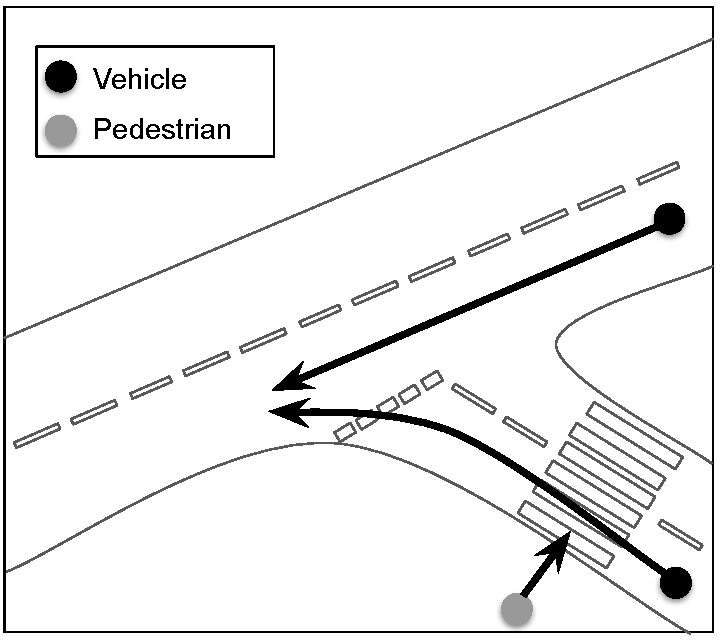
\includegraphics[width=1\textwidth]{Other/Figures/TestCasesDiagramV2_a.pdf}
        \caption{}
        \label{Test_a}
    \end{subfigure}
    \begin{subfigure}{.24\textwidth}
        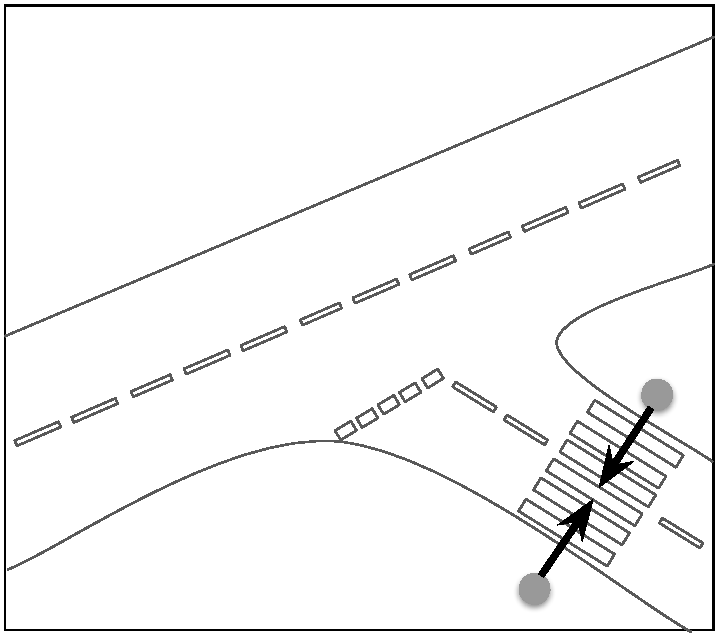
\includegraphics[width=1\textwidth]{Other/Figures/TestCasesDiagramV2_b.pdf}
        \caption{}
        \label{Test_b}
    \end{subfigure}
    \caption{Schematic of test scenarios for (a) Tests 1-4, (b) Tests 5-6. Descriptions are given in Table~\ref{TableOfExperiments}.}\label{f:test_a_and_b}
\end{figure}

This case study draws on a setup used to verify an urban mobility and transport solution, where the primary verification objective is to test the behaviour of an ego vehicle in an urban environment at a T-junction in response to pedestrians and other vehicles.
%
Thus, the scene for our investigation is the T-junction with the scenarios as shown in Figure~\ref{f:test_a_and_b}.

This scene was used to create a number of scenarios involving pedestrians and vehicles in order to identify any changes in the actor paths over repeated tests executed under a variety of systematically designed conditions and hence study any simulation variance.
%
The vehicles and pedestrians were given trajectories, via pre-defined waypoints, that would result in either colliding with or avoiding other actors.
\todo[inline]{Decide past or present tense and be consistent throughout.}


\todo[inline]{Set the threshold, explain what a good threshold is, available options and what was selected and why.}



\subsection{Tolerable Simulation Variance}

\todo[inline]{Terminology:\\
{\bf Accuracy} is the degree of closeness/conformance to a known value.
\\
{\bf Precision} is the ability to get a particular value several times, i.e.\ repeatability of a measurement.
\\
{\bf Tolerance} is the allowable or predictable deviation from a known/desired value, e.g.\ $\pm 1cm$. 
\\
See {\small\url{https://www.starrapid.com/blog/designing-for-manufacturing-accuracy-precision-and-tolerance/}} for further details.
}

% \todo[inline,color=green!40]{GC addition: Ideally simulation results should be precise, where repeated tests give exactly the same result.}

To achieve stable verification results over repeated test runs, the simulated actor states must be precise to a specific tolerance.
%
Deterministic behaviour would result in zero variance of the simulated actor states but if this cannot be achieved then what is permissible?
%
% \todo[inline,color=green!40]{GC addition: Deterministic behaviour would result in zero tolerance of the simulated actor states but if this cannot be achieved then what is a permissible tolerance? }
%
The tolerance must be appropriate to allow accurate assertion checking and coverage collection in the simulation environment, but not so small as to fail with minor computational perturbations. {\color{red} {\sc What would fail?}}
%
Thus, a tolerance must be defined to reflect the precision at which repeatability of simulation execution is required. 

% tolerances are controlled to within a small, acceptable degree of variability from one part to another.
%
% but a larger value may be acceptable for non-urban environments, e.g. motorway or highway. Similarly, the threshold value should not be so small as to fail with minor computational bottlenecks, e.g. $1\mu m$.
% 
% To determine if the ego vehicle performs correctly, i.e.\ does not violate assertions, t

% The autonomous vehicles operating in the last-mile mobility and delivery sector as considered in this case study will predominantly operate within urban rather than highway or motorway environments. 
%
For this case study a tolerance on actor position of $1$m would be insufficient when considering the spacial resolution required to distinguish between a collision and a near-miss event. 
%situations such as potentially dangerous close passing of a cyclist. 
A very small value, e.g.\ $1\times10^{-12}m$, may be overly-sensitive to minor computational perturbations and generate false positives. 
% due to the simulation \textit{noise floor}\footnote{See Fig.~\ref{CarsCollisionCG25}.} 
Therefore, for this case study and, more broadly, for our general verification requirements, a tolerance of $1$cm has been selected. 
% Thus any variation of less than $1$cm is tolerable. 
Thus any variance of less than $1$cm is permissible. To put this another way, we can accept a precision with a tolerance of $\leq$$\pm$1$cm$. 


% considered to be sufficient for assertion checking in urban environments. 
%
% A value larger than this, e.g. $1m$ will not be sufficient to spatially resolve these scenarios and a smaller value, e.g. $1mm$ may result in false positives.

% \todo[inline]{Move to Case Study, rewrite with justification: Two autonomous vehicle projects this group are involved in, Robopilot and Capri, are looking at urban mobility and last mile delivery solutions which are predominantly concerned with urban environments rather than highway or motorway scenarios. Because of this, a deterministic threshold of $1m$ is insufficient when considering potentially dangerous close passing of cyclists and pedestrians and therefore a threshold of $1cm$ is more suitable.} \todo[inline]{Formal writing, no reference to the group or project, please.}

\todo[inline,color=red!40]{old: For the simulation to be considered repeatable, the overall level of simulation variance for any actor should be less than a user-defined threshold, or \textit{permissible tolerance}, for a given scenario and verification objective.  }

% \todo[inline,color=green!40]{GC question: should we remove this line below as it is repeating above statement?}
In the following, case study results are shown in terms of the maximum deviation, $\max\sigma$, from the mean actor path over the entire simulation history where any value higher than the specified tolerance is considered non-permissible.
%
\todo[inline,color=green!40]{GC edit: Case study results are shown in terms of the maximum deviation, $\max\sigma$, from the mean actor path over the entire simulation history %and the deviation threshold in this investigation is $1cm$, 
where any value higher than the specified tolerance is considered non-permissible. }

% ***************************************************
%  Actor Collisions
% ***************************************************


\subsection{Actor Collisions}\label{S:Actor_Collisions}
Previous investigations into the Unreal Engine indicated that collisions between dynamic actors {\color{red} Why DYNAMIC?} and solid objects, termed \textit{blocking physics bodies} in Unreal Engine documentation~\cite{collision_overview}, can lead to high simulation variance~\cite{TSLUnrealEngineTesting}. {\color{red} NOT ACCESSIBLE}
%
Collisions and the subsequent physics calculations that are processed, termed \textit{event hit} callback in Unreal Engine, were identified as potentially key aspects to the investigation into simulation variance.

The tests used for the case study are listed in Table~\ref{TableOfExperiments}. They cover a range of interactions between actor types. 
%
Tests 1 \& 2 involve two vehicles meeting at a junction where they either do not collide (Test 1) and where they do collide (Test 2), thereby triggering an \textit{event hit} callback in the game engine. In both cases the trajectories of the vehicles are hard-coded to follow a set of waypoints spaced at $0.1$m 
% \todo[inline]{AG: is this value correct or should it be 2.0m? AG-reply: The granularity of the trajectory waypoints is 0.1m, but the lookahead distance that the actors use is 2m ... actors would ignore trajectory waypoints that are less than 2.0m away from them.} 
intervals using a PID controller. 
%
In Test 3 a mixture of different actor types is introduced where two vehicles drive without collision and a pedestrian walks across the road at a crossing point. 
%
In Test 4 this pedestrian collides with one of the vehicles at the crossing, triggering an \textit{event hit} callback, see Fig~\ref{Test_a}. Similar to vehicles, pedestrians navigate via a set of regularly spaced waypoints at $0.1$m intervals using the A* algorithm which is the default controller for the CARLA pedestrian actors. Tests 5 \& 6 involve only pedestrians that either do not collide (Test 5) and that do collide (Test 6), see Fig.~\ref{Test_b}. 

\todo[inline]{Again, match the flow diagram steps in the subsections, but here wrt the case study steps.}

% ***************************************************
%  Experiment Description
% ***************************************************
\subsection{Evaluation Metric}\label{s:Experiment_Description}
% \todo[inline]{Say what needs to be logged, what needs to be calculated based on these logs and what one should be looking for and why.}
For each test the position of each actor is logged at $0.1s$ intervals providing a trace of that actor's path with respect to simulation time. 
%
The logs from repeated tests are compared at the same time index $t$ for each actor $a$ to provide a value for the variance of actor $a$ at time index $t$, $\sigma_a^{2}(t)$, at each point in time. {\color{red} This gives a variance function over time for each actor.}

{\color{blue} The logs from repeated tests are sourced to establish a value for the variance associated with each actor, $a$, at each time point $t$, giving a variance function over time for each actor, $\sigma_a^{2}(t)$.}

Herein the results are given in terms of the deviation, $\sigma_a(t)$, which indicates the dispersion of the actor position data relative to the mean and is helpfully in the same units as actor position, i.e.\ metres ($m$), for ease of interpretation.
%
\todo[inline,color=green!40]{GC Addition: For each test the position of each actor was logged at $0.1s$ intervals providing a trace of that actor's trajectory with respect to simulation time. 
%
Repeated traces are compared at the same time index $t$ for each actor $a$ to provide a value for the variance, $\sigma_a^{2}(t)$. 
%
Herein the results are given in terms of the deviation, $\sigma_a(t)$, which indicates the dispersion of the actor position data relative to the mean and is helpfully in the same units as actor position, $m$, for ease of interpretation. }

The maximum variance over the entire set of $n$ simulations is therefore defined as the largest variance of any actor at any time in the simulation, as given in Equation~\ref{eq:max_sigma}. {\color{red} This is still a function over time - should it be?}
\begin{equation} \label{eq:max_sigma}
\max_{a,t}\sigma_a^{2}(t)
\end{equation}
The maximum deviation is the square root of the maximum variance {\color{red} The absolute value of the square root?} and herein referred to as ${\max\sigma}$ for brevity. {\color{red} So, ``a'' is any actor or a specific actor? Likewise, ``t'' is any time point or a specific time point? NOTE that any actor any time means a in A and t in T, where A is the set of actors and T is the set of all time points.}

The maximum deviation, $\max\sigma$, was analysed against the different scenarios and settings that were identified as potential sources of non-determinism, and compared against the limit of \textit{permissible variance} to indicate if the simulation was reliable for verification purposes.
% The output for each experiment can therefore be summarised as the \textit{maximum variance} of any actor over the $n$ repeated tests. 
% The maximum, rather than average, variance is chosen to indicate the worst case where an average could obscure outlier data points when a high number of repeated tests are performed. 
\todo[inline,color=green!40]{GC Addition: The maximum deviation, $\max\sigma$, was analysed against the different scenarios and settings that were identified as potential sources of non-determinism, and compared against the threshold of \textit{permissible tolerance} to indicate if the simulation was reliable for verification purposes. } 
%
% Preliminary work\footnote{see footnote 14} suggested that adding stress to the CPU or GPU will contribute towards increased . 
% \todo[inline]{Introduce the need to use CPU and GPU HW in a game engine or any simulation HW. GC done}


% Once the experiments are run, the logged data is post processed to find the variance in the logged data between the different runs. Note that bifurcation effects can cause a jump in the variance, so it is worth plotting the different logged paths in order to determine if there are any bifurcation effects.

% This whole process is repeated for various internal and external settings (if needed). 
% Then various plots can be created to draw the engine's simulation variance. 
% Thereon, it would be up to the verification engineers to determine where they want to define the line below which the simulation variance would be acceptable, and thus know at which levels of computational utilisation they can guarantee to run repeatable experiments.   

% ***************************************************
%  Internal Settings
% ***************************************************
\subsection{Internal Settings}

Within Unreal Engine there are numerous internal settings relating to the movement and interaction of physical bodies in the simulation. Settings can be adjusted to alter how actors interact and path plan via the navigation mesh of the environment, e.g.\ \textit{Contact Offset} and \textit{Navmesh Voxel Size}, or can be changed to improve the fidelity of physics calculations between game update steps, e.g.\ \textit{Physics Sub-Stepping} and \textit{Max Physics Delta Time}. Other options such as \textit{Enable Enhanced Determinism} were investigated along with running the engine from the command line with options for more deterministic behaviour \texttt{-deterministic}, floating-point control \texttt{/fp:strict} and headless mode \texttt{-nullrhi} along with running the test as a packaged release by building and cooking~\cite{releasing_project}.
% \todo[inline]{Maybe we can introduce our initial study here? Picture of the man and moving bloack and a result showing the path traces in x,y etc?}
An initial study into the Unreal Engine using a pedestrian and a moving block was used to investigate simulation variance against these settings. The results were compared to a baseline of the default engine settings. 
%
However, none of these options improved simulation variance significantly and all internal setting were set restored to the default values. Details on this previous investigation can be found on the Trustworthy Systems GitHub~\cite{TSLUnrealEngineTesting}. {\color{red} NOT ACCESSIBLE}



% ***************************************************
%  External Settings
% ***************************************************
\subsection{External Settings}
% \todo[inline]{This would be ``External Settings'' and can be introduced after finding that internal settings alone did not tame the non-determinism. :(}

After discovering that internal engine settings could not achieve a simulation variance that met the required 
% \textit{deterministic threshold}, 
\textit{tolerance}, {\color{red} WHEN HAS THIS BEEN REPORTED?}
settings external to the game engine were explored. 
%
Game engines, and simulation hardware more generally, will utilise available system resources such as central and graphical processing units (CPU and GPU respectively), to perform physics calculations and run the simulation environment. 
%
For high performance simulations the demand on these resources may be a significant fraction of the total available and an initial hypothesis was that as this ratio tended toward one, there would be an increase in \textit{simulation variance}. This hypothesis was supported by our initial work performed on the unreal engine~\cite{TSLUnrealEngineTesting} and was explored more fully in this work using the CARLA platform. {\color{red} From a reviewer's point of view this is a mysterious initial study that has been referred to often but nothing has been presented. Either take out or include, at least wrt.\ the overall observations, such as the support for this hypothesis.}

To replicate in a controlled manner the high computational loads that may be anticipated for high performance simulations, software that artificially utilises resources on both the CPU and GPU were executed alongside the simulation. 
%
% In order to reproduce conditions for computationally intensive simulations, the experiments are executed with additional levels of artificial resource utilisation. 
Resource utilisation was artificially increased for both CPU and GPU devices to include a range of values from 0 to 95\% (see Section~\ref{s:methodology}) using reported values of the system monitors \texttt{htop} and \texttt{nvidia-smi} respectively. Resource utilisation figures reported here should be considered approximate values.
% The level of additional resource utilisation, above that of the needs of the simulation, was increased from $0\%$ (no additional resource load) in $25\%$ increments up to a maximum of $95\%$ for both CPU and GPU as reported by system monitors (\texttt{htop} and \texttt{nvidia-smi} respectively). 

\todo[inline,color=green!40]{GC Addition (para below):} 
%Issues around floating-point precision and concurrency as previously mentioned notwithstanding, 
Practitioners should also be aware that many libraries for calculating variance itself may require attention to get precise results. For example the \texttt{numpy} method of variance is sensitive to the input precision and will return an incorrect answer if the wrong parameters are set~\cite{NumpyVar}. In \texttt{matlab}, the calculation of variance may switch from single thread to a multi-threaded execution not obviously apparent to the user when the input data size becomes large enough, opening up the potential for concurrency-induced imprecision~\cite{matlab_parallel_computing}. 

\begin{figure}[t]
    \centering
    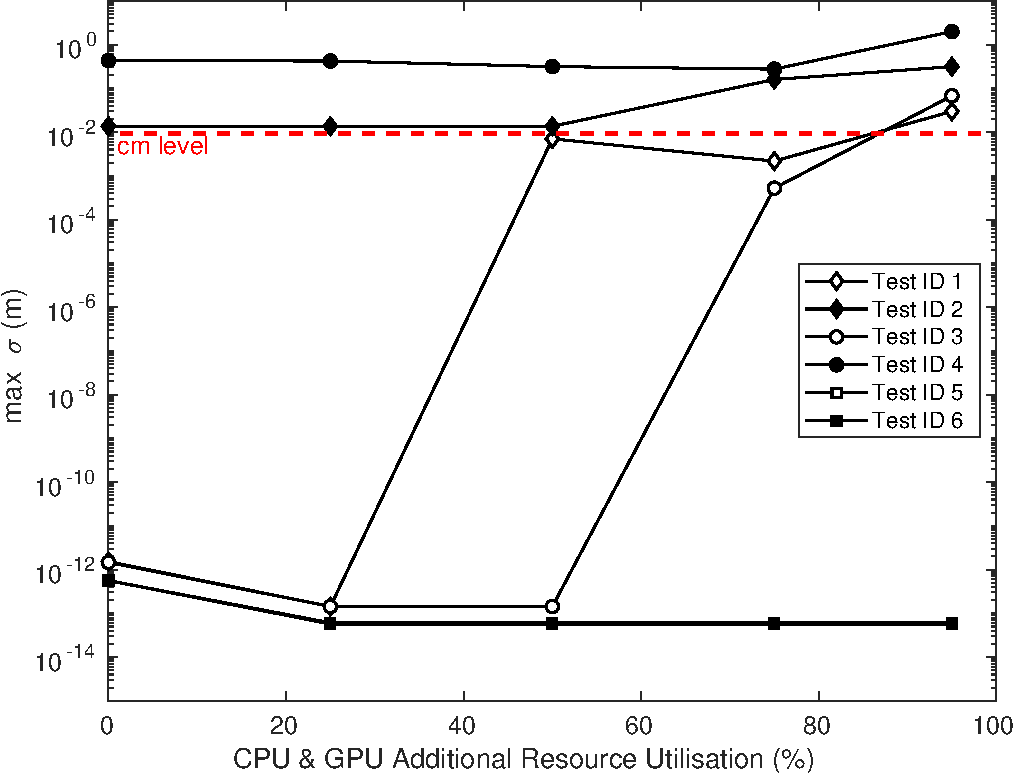
\includegraphics[width=0.48\textwidth]{Other/Figures/ExperimentsStressSummaryV5.pdf}
    \caption{Summary of results showing maximum deviation for each scenario against different resource utilisation levels. Tests 5 and 6 overlap having almost identical results.}
    \label{ExperimentsStressSummary}
\end{figure}
	
% ***************************************************
%  System Configuration and Screening
% ***************************************************
\subsection{System Configuration and Screening}\label{s:screening}
These tests were carried out on an Alienware Area 51 R5 with an i9 9960X processor with 64GB non-ECC DDR4 RAM at 2933MHz with an NVIDIA GeForce RTX 2080 GPU with 8GB GDDR6 RAM at 1515 MHz. 
%
Operating systems was Linux Ubuntu 18.04.4 LTS. To ensure reliability of results, each test was repeated 1000 times. 
%
Tests were carried out in CARLA (v0.9.6 and Unreal Engine v4.22) using synchronous mode with a fixed $dt$ of $0.05$s. 
%
A detailed guide for reproducing these experiments along with the scripts used are provided on github\footnote{\url{https://github.com/TSL-UOB/CAV-Determinism/tree/master/CARLA_Tests_setup_guide}}.
%
To eliminate some of the potential sources of non-determinism outlined in Section~\ref{s:nondeterminisimSources} a series of screening tests and analyses were performed on our system. These were:

\begin{itemize}[leftmargin=*]
    \item System memory: \texttt{memtest86}~\cite{MemTest86} full suite of tests ran, all passed.
    \item Graphical memory: \texttt{cuda\_memtest}~\cite{cuda_memtest}\cite{shi2009testing}.
    \item Non-uniform memory access: \texttt{numactl}~\cite{numactl_NUMA} was used to fix the simulator and test script to single cores but only a minor (2\%) improvement in simulation variance was observed and therefore not used for subsequent testing.
\end{itemize}





% Given that our interest is on AV simulations, this study presents a number of experiments run on typical agents used in AV simulations and their interactions with each other. These agents are classified into two, either vehicles(cars, motorcycles, bikes etc.) or pedestrians (can include animals). Here we will walk through our hypothesis, description of our tests and the analysis of results from the different tests. We will point out at each stage where we sit in Figure~\ref{method_diagram} as we go through this case study.    

% \subsection{Problem And Hypothesis}
% We want to see whether using Unreal Engine 4 (UE4) along with CARLA \cite{CARLA_paper} for V\&V of AV simulations is deterministic or not; if not then what is the simulation variance that we will operate with, is it acceptable or not, and whether it worsens with stressing GPU and CPU.

% Our hypothesis is that since UE4 is a game engine it is non-deterministic, however, the simulation variance would be very low to acceptable limits that allows verification engineers to use it confidently and assume that tests would be repeatable. This behaviour is expected not to hold as the level of computing stress increases.     


 % targetting the closest waypoint but ignoring any waypoints closer than a fixed \textit{look-ahead distance} ($d_l$)\footnote{Targeting waypoints with $d_l<0.4$ tend to cause improper navigation with the implemented PID controller}.
% Pedestrians have the functionality of dynamic path planning i.e. they can avoid obstacles to reach their waypoints and so they can avoid static objects and other actors. To ensure they intersect (collide) with each other $d_l$ is altered; the smaller the look ahead distance the less chance the pedestrian will get to path plan around each other, and thus making sure they intersect. (This sounds like at some $d_l$ the pedestrians do not collide - is this true?) 


% Similar to the vehicle actors, the look ahead range ($d_l$) can be modified so that the actor is forced to navigate on waypoints that are further away. In test 7 $d_l$ is increased from $0.4m$ to $2.0m$ and in test 8 to $20m$ which was done to investigate if the path planning algorithm was deterministic when given waypoints further ahead.

% The vehicles in this simulator follow a trajectory of waypoints using a PID controller and they have a look ahead distance that they target for from a given list of trajectory waypoints. Similarly with the pedestrians, but they don't have a PID controller and they can do dynamic path planning using A* algorithm to reach their destination or in this case a trajectory waypoint.

% Starting from step 1 in the methodology diagram (Design Experiment); we are using a double mini roundabout for our experiments. 

% The list of tests shown in Table \ref{TableOfExperiments} were chosen to cover the mandatory interactions between the different types of agents. These are summed up in the following: \textbf{i)}Agents (vehicles and pedestrians) moving with no collisions or interactions with each other \textbf{ii)}Collision between vehicles \textbf{iii)}Collision (intersection) between pedestrians \textbf{iv)}Collision between vehicles and pedestrians.


% Tests 1, 3and 5 are similar and there are no collisions in them, they were done as separate tests (instead of combining them into one) for the sake of simplicity and to use them as base lines for the tests-collision versions of them. The tests for collisions and non-collisions differ by a very slight change in the trajectory of the agents just to make them avoid colliding or intersecting with each other.

% Test 2 is a collision between two vehicles and no pedestrians involved and is depicted by \ref{Test_a}, where the two vehicles will approach the roundabout and crash.

% Tests 6,7 and 8 are tests with pedetrians having the same trajectory waypoints but walking in opposite directions to each other (see Figure~\ref{Test_b}). 
% Pedestrians have the functionality of dynamic path planning i.e. they can avoid obstacles to reach their waypoints and so they can avoid bumping into each other. Hence, to make sure they intersect (collide) with each other then we  have set tests 6,7 and 8 to be the same but with different look ahead distances; the smaller the look ahead distance the less chance they will get to path plan around each other, and thus making sure they intersect.

% In V\&V of AV simulations, collisions of pedestrians together is not of much interest, nevertheless we decided to include these tests for the sake of completeness and to obtain a full image of the simulation variance of the simulator.

% Test 4, is where a vehicle hits a pedestrian and runs over it on a zebra line, as shown in Figure~\ref{Test_a}.

% Proceeding to step 2; there is about 20 different internal settings related to our context that can be tweaked in UE4; such as \textit{Enable Enhanced Determinsim}, \textit{PhysX Tree Rebuild}, \textit{Max Physics Delta Time} etc. By doing various inspections around them we did not notice much improvement or worsening in the simulation variance between test runs, therefore the internal settings option was disregarded. However, one of the options we used is synchronus mode with a fixed time step that is available in CARLA. This would make the simulator proceed to the next tick only when commanded to do so by our script, which makes runs' flow more consistently.  

% On the other hand the external settings (step 3), where CPU + GPU are stressed, did show significant variations in the results as will be discussed in section \ref{ResultsSection}. Different levels of stress were applied to the computer; using the \texttt{stress} function \cite{CPU_stress} to stress the CPU and \texttt{gpu-burn} from github \cite{GPU_stress} to stress the GPU.

% In terms of running the experiments (step 4), \textbf{i)} the computer used is an Alienware Area 51 R5 with an i9 9960X CPU chip, NVIDIA GeForce RTX 2080 graphics card and 64GB of RAM; \textbf{ii)} \texttt{nvidia-smi} and \texttt{htop} were used to monitor the levels of GPU and CPU stress respectively before and while the experiments were executed \cite{monitoring_stresses}; \textbf{iii)} the computer was 



\begin{figure*}[t]
    \centering
    \begin{subfigure}{.49\textwidth}
        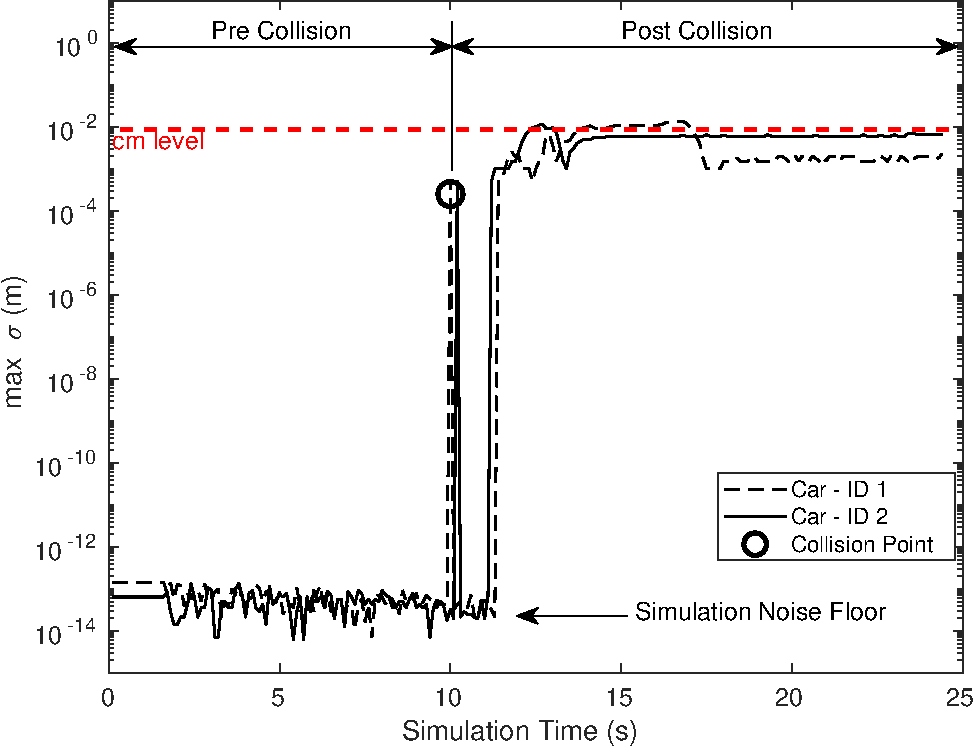
\includegraphics[width=1\textwidth]{Other/Figures/CarsCollisionCG25_V4.pdf}
        \caption{}
        \label{CarsCollisionCG25}
    \end{subfigure}
    \begin{subfigure}{.49\textwidth}
        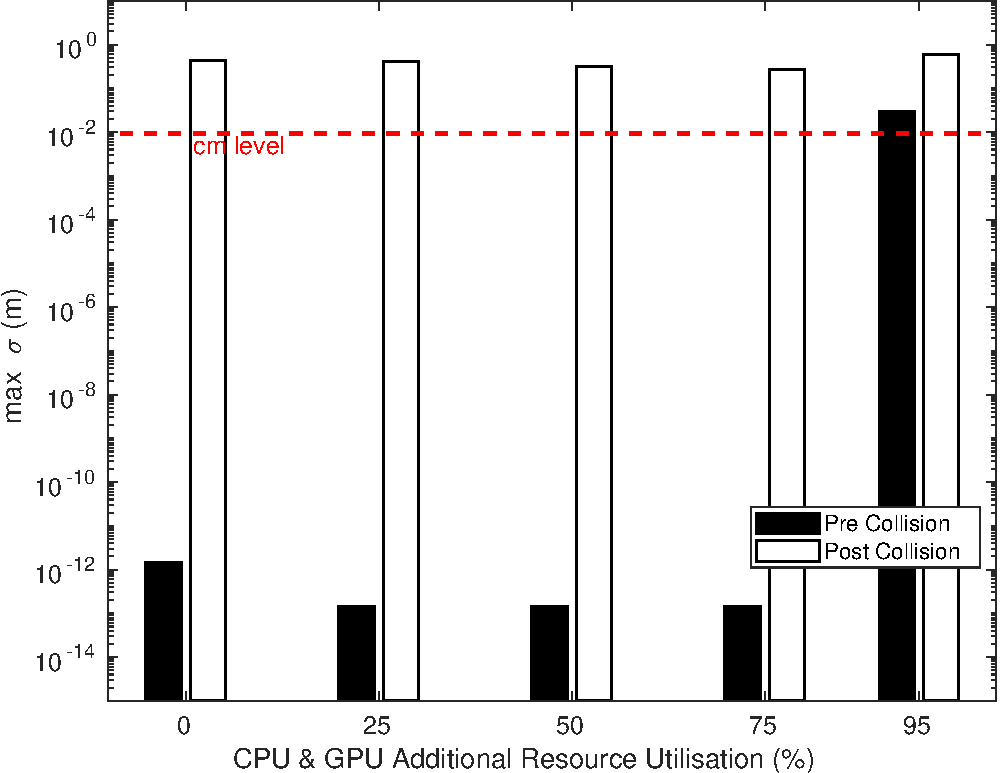
\includegraphics[width=1\textwidth]{Other/Figures/CarsCollisionPrePostV5.pdf}
        \caption{}
        \label{CarsCollisionPrePost}
    \end{subfigure}
    \caption{Vehicle to vehicle collision (test 2) showing (a) maximum deviation against simulation time for 25\% resource utilisation and (b) maximum deviation pre- and post-collision against resource utilisation. The simulation noise floor is shown in (a) which is the empirical lower limit of deviation for the hardware reported in this study.}
\end{figure*}


% ***************************************************
%  Results and Discussion
% ***************************************************
\subsection{Results and Discussion}\label{ResultsSection}
A summary of all the results are shown Table~\ref{TableOfExperiments} in the column $\max\sigma$ (unrestricted), where the value reported is the maximum deviation across all resource utilisation levels, i.e. the worst case for a given scenario.  
%
From these  results it is clear that scenarios with only pedestrian actors (tests 5-6) display results within tolerance over all resource utilisation levels with or without a collision where $\max\sigma$ is $5.6\times10^{-13}$ or $0.56\si{\pico\metre}$. However, all other scenarios involving vehicles or a mixture of actor types breach the tolerance that has been set, with some deviation in actor path as large as $59$cm.
\todo[inline,color=green!40]{GC Edit: From these  results it is clear that scenarios with only pedestrian actors (tests 5-6) display results within the permissible tolerance over all resource utilisation levels with or without a collision where $\max\sigma$ is $5.6\times10^{-13}$ or $0.56\si{\pico\metre}$. However, all other scenarios involving vehicles or a mixture of actor types breach the permissible tolerance that has been set, with some deviation in actor path as large as $59$cm. }
%
Clearly a deviation in results of such a large amount is unacceptable if simulation is to be used as a reliable verification tool.

Resource utilisation level was found to have a significant impact on \textit{simulation variance}.
%
Figure~\ref{ExperimentsStressSummary} shows $\max\sigma$ against the artificially increased resource utilisation level, where the $x$-axis indicates the approximate percentage of resource utilisation (for CPU \& GPU). In this figure, anything above the $1$cm level (dashed line) is considered non-permissible according to our specific tolerance level informed from our verification requirements.
%
\todo[inline]{Where are the verification requirements listed? They should be part of the scenario description. GC- added to the start of section 3.} 
%

A general pattern in the results indicates that; some scenarios consistently fail to produce results within permissible levels of variance at any resource utilisation level (Fig.~\ref{ExperimentsStressSummary} Test ID 2 \& 4 above the dashed cm level), some are consistently within tolerance (Test ID 5 \& 6 with pedestrians only), and that some cases only fail to meet the tolerance requirement when at higher utilisation levels, breaching the tolerance above 75\% resource utilisation (Test ID 1 \& 3).

\todo[inline]{Help the reader see what you can see by explaining exactly where this can be seen in the figure(s). GC text added above}




However, the non-permissible results in Figure~\ref{ExperimentsStressSummary} (all those above the dashed line) are the worst case account of the situation, as per Equation~\ref{eq:max_sigma}, as the maximum variance is taken over the entire simulation period.

Examining specifically the results from tests 2 \& 4 as a function of simulation time reveals further information about the simulation variance before and after an actor collision. Fig.~\ref{CarsCollisionCG25} shows this examination for vehicle to vehicle collisions (test 2), where $\max\sigma$ switches from permissible prior to the vehicle collision to non-permissible post-collision. 
%
This pattern of permissible results prior to collision and non-permissible post-collision is maintained up to a resource utilisation level of approximately 75\%, see Fig.~\ref{CarsCollisionPrePost}. This time series examination was repeated for vehicle to pedestrian collisions (test 4) and the results are shown in Fig.~\ref{CarsPeopleCollsionsCG25}. Similarly to vehicle-to-vehicle collisions, the variation of $\max\sigma$ for vehicle to pedestrian collisions indicates permissible pre-collision behaviour with up to 75\% resource utilisation, see Fig.~\ref{CarsPeopleCollisionPrePost}. This is a key finding of this work; it suggests that verification engineers should consider terminating tests at the point of a collision, as any post-collision results will be non-permissible.
\todo[inline,color=green!40]{GC Edit: Examining specifically the results from tests 2 \& 4 as a function of simulation time reveals further information about the simulation variance before and after an actor collision. Fig.~\ref{CarsCollisionCG25} shows this examination for vehicle to vehicle collisions (test 2), where $\max\sigma$ switches from permissible prior to the vehicle collision to non-permissible post-collision. 
%
This pattern of permissible results prior to collision and non-permissible post-collision is maintained up to a resource utilisation level of approximately 75\%, see Fig.~\ref{CarsCollisionPrePost}. This time series examination was repeated for vehicle to pedestrian collisions (test 4) and the results are shown in Fig.~\ref{CarsPeopleCollsionsCG25}. Similarly to vehicle-to-vehicle collisions, the variation of $\max\sigma$ for vehicle to pedestrian collisions indicates permissible pre-collision behaviour with up to 75\% resource utilisation, see Fig.~\ref{CarsPeopleCollisionPrePost}. This is a key finding of this work; it suggests that verification engineers should consider terminating tests at the point of a collision, as any post-collision results will be non-permissible. }
% \todo{Why ``not reliable''.} 

\begin{figure*}[h]
    \centering
    \begin{subfigure}{.49\textwidth}
        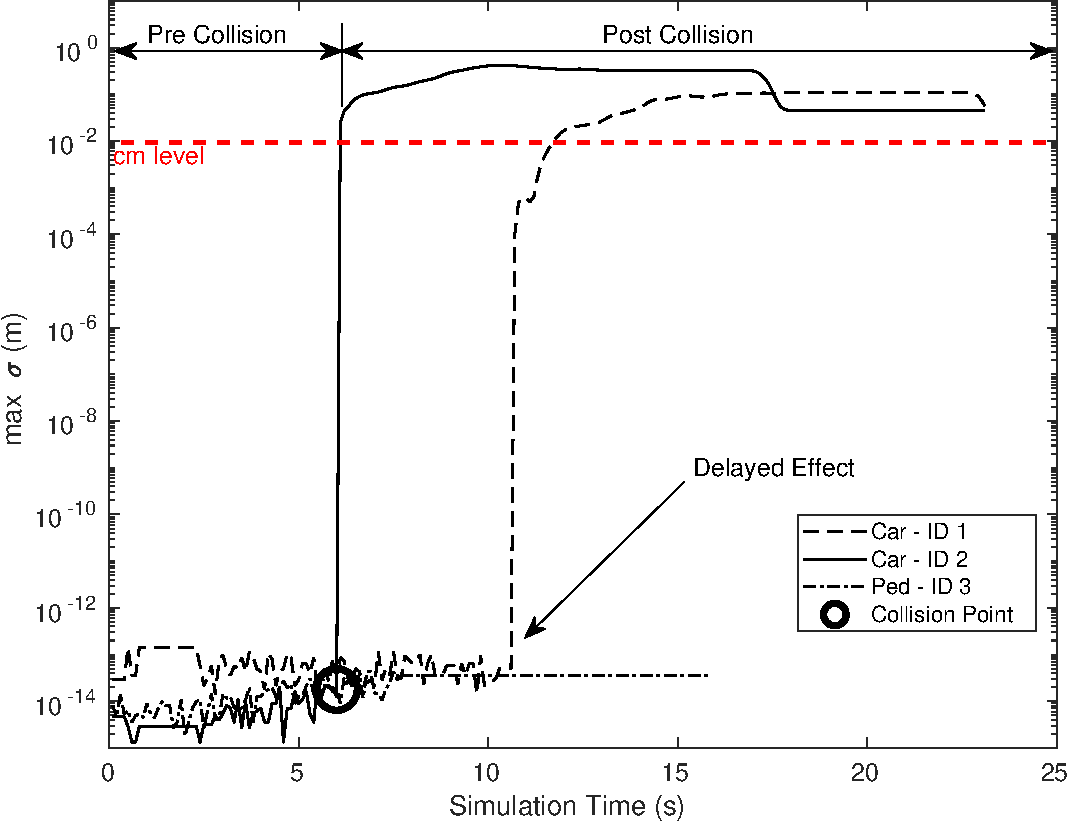
\includegraphics[width=1\textwidth]{Other/Figures/CarsPeopleCollsionsCG25_V3.pdf}
        \caption{}
        \label{CarsPeopleCollsionsCG25}
    \end{subfigure}
    \begin{subfigure}{.49\textwidth}
        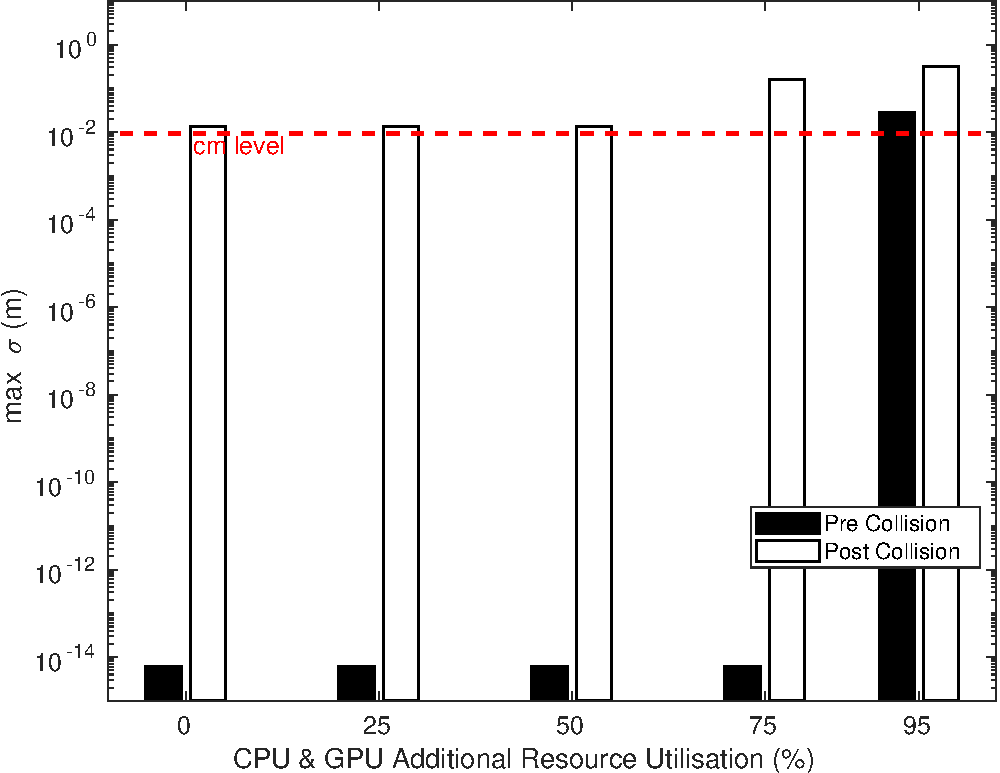
\includegraphics[width=1\textwidth]{Other/Figures/CarsPeopleCollisionPrePostV5.pdf}
        \caption{}
        \label{CarsPeopleCollisionPrePost}
    \end{subfigure}
    \caption{Vehicle to pedestrian collision (test 4) showing (a) maximum deviation against simulation time for 25\% resource utilisation and (b) maximum deviation pre- and post-collision for different resource utilisation levels.}
\end{figure*}

\begin{figure}[t]
    \centering
    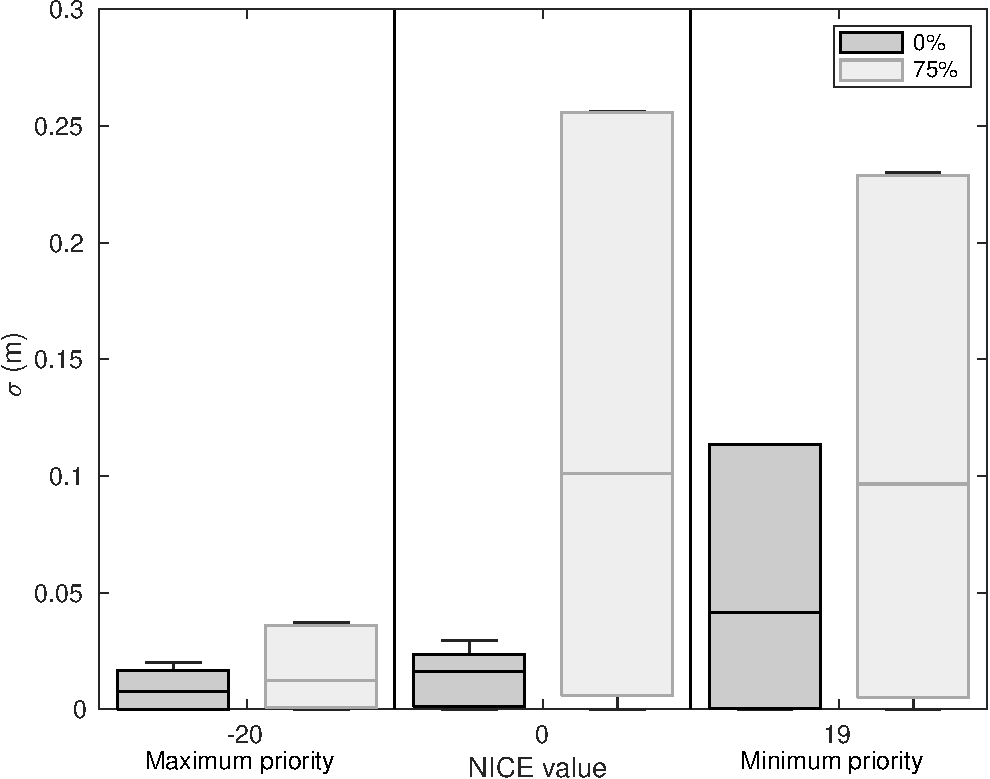
\includegraphics[width=0.48\textwidth]{Other/Figures/NICE_analysis_summary_V4.pdf}
    \caption{Summary of investigating the effect of NICE priority setting for 0\% and 75\% additonal CPU \& GPU resource utilisation.}
    \label{NICEExperimentStressSummary}
\end{figure}


The second key finding of this work is illustrated in Fig.~\ref{CarsPeopleCollsionsCG25}. In this scenario (test 4), there is a collision between a vehicle (Car ID 2, solid line) and a pedestrian (Ped ID 3, dot dash line) which occurs at a simulation time of approximately $6$s and a second vehicle actor (Car ID 1, dashed line), which is \textit{not involved in the collision}. There are three observations here; firstly that the vehicle directly involved in the collision (Car ID 2) displays high simulation variance immediately after the collision.
% as described above. 
Secondly, that the maximum deviation of the pedestrian involved in the collision (Ped ID 3) is at a tolerable level throughout the test\footnote{However, please note that in CARLA the pedestrian object is destroyed post-collision hence the flat line from $t=6$s onwards.}. Thirdly, we observed a delayed effect on Car ID 1 showing high simulation variance with a $5$s delay \textit{even though this vehicle was not involved in the collision}. This final point should be of particular concern to verification engineers and research practitioners in the field as it implies that \textit{any collision between actors can affect the simulation variance of the entire actor population} and could potentially result in  erroneous assertion checking.

% \todo[inline]{Make sure that assertion checking has been introduced before.}

% \textbf{Strange gap post-collision for few seconds}

% \textbf{Should we rename 'test' to 'scenario???'}

% \todo[inline]{Big question why does high-RU influence simulation variance?? Can we tie this to thread scheduling and will NUMAclt change this conclusion?'}

% Scenarios that include both collisions and vehicle actors were non-deterministic. However, when observing the deviation in actor paths against simulation time, Fig.~\ref{CarsCollisionCG25}, the simulation is deterministic prior to collision but not afterwards. 

% This was calculated by averaging the variance between all of the different runs through out the simulation time for all of the agents, then taking the square root to obtain the total mean devaiton. Note the dotted red line in the plot shows the millimeter (mm) level. Below this level we assume that the simulation variance is low enough that it would not affect our assertion checking for V\&V of AV simulations purposes, that it is sufficient to assume the tests are deterministic and repeatable. This line can be moved up or down and it is entirely up to verification engineers where they want to define the level below which tests' variance is negligibale and it is suffcient to assume that tests are deterministic.
%
\begin{figure*}[t]
    \centering
    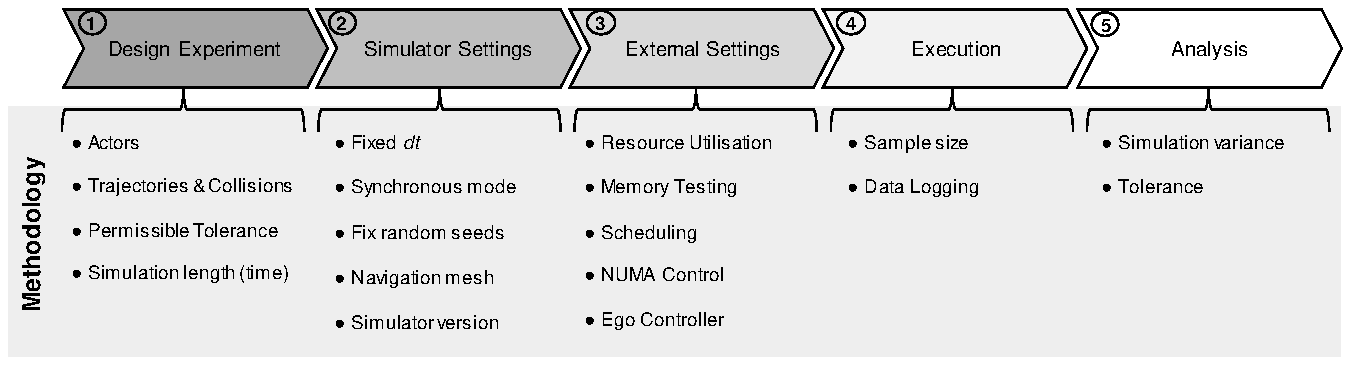
\includegraphics[width=0.99\linewidth]{Other/Figures/Methodology_Diagram_v5.pdf}
    \caption{Flow diagram of the methodology proposed to determine the simulation variance of a simulation.}
    \label{method_diagram}
\end{figure*}

\todo[inline]{Sum this up and lead on to the Methodology - assuming that this section is placed before the Methodology section. This should cover that our results are clearly specific to our HW and provide evidence of non-determinism, but the results are not transferable. Thus, we present a general Methodology that others can re-use/apply to determine whether or not their sim is deterministic - in the next section.}
 
The main findings of this work suggest a working practice that would minimise the non-deterministic effects observed in this investigation. By limiting simulation results to pre-collision data and ensuring resource utilisation levels do not exceed 75\%, the permissible variance of $1$cm is achievable as shown in the \textit{restricted} column in Table.~\ref{TableOfExperiments}. By applying this set of restrictions upon the simulation the maximum observed deviation across all experiments was $0.98$cm which is within the target tolerance we set out to achieve. 
%
Practitioners may wish to set a stricter resource utilisation level, such as less than 50\% to further reduce the potential dispersion of results if this is required for their chosen application. 
%
\todo[inline,color=green!40]{GC Addition: Practitioners may wish to set a stricter resource utilisation level, such as less than 50\% to further reduce the potential dispersion of results if this is required for their chosen application. 
%For this case study a 50\% restriction of resource utilisation would reduce deviation across all experiments to XXX.XXXmm. 
}

\subsection{Process Scheduling Priority}
An investigation into the response of process scheduling on the simulation variance was undertaken. The experiment was repeated ($n=1000$) using test 1 but altering the process scheduling priority using the program \texttt{NICE}.\footnote{\url{http://manpages.ubuntu.com/manpages/bionic/man1/nice.1.html}} Setting a higher priority for the simulator process with respect to the resource utilisation processes, it was possible to determine if scheduling could account for the increased simulation variance when the system is under high resource utilisation.
%
To give a process a high priority a negative NICE value is set with the lowest being -20. To decrease the priority a positive value is set, up to +19. The default NICE value is 0.

The results are presented in Fig.~\ref{NICEExperimentStressSummary} where the box denotes the inter-quartile range, non-outlier limits by the whiskers and a horizontal bar for the median. The figure shows that decreasing the priority (right hand side of plot) has little effect on simulation variance when compared to a NICE value of 0 (central plot bars). Increasing priority (left hand side of plot) reduced variance for the 75\% resource utilisation but this did not account for all the difference in the observed results. This is demonstrated in the maximum priority setting where the bars in plot are not equal, indicating an additional contribution to variance not accounted for by the NICE scheduling. 
%
This unaccounted difference in the variance may be due to the lack of absolute control that \texttt{NICE} has over the process scheduling.\footnote{\url{https://askubuntu.com/questions/656771/process-niceness-vs-priority}}

\subsection{Investigation Summary} \label{s:empirical_summary}

% \todo[inline]{GC-need to reference the 'restricted' set of results here too}

\todo[inline]{Do we need to say here why we think certain results are non-det, what the reasons might be?? The results indicate that actor type, resource utilisation and collision events all affect the determinism in the CARLA simulator. Collision events may utilise more computational resources than simulations without such events, i.e. the physics loop takes longer to process as there are complex physical interactions to resolve. This may coincide with the second observation that higher resource levels also lead to non-deterministic results. We hypothesise that both these observations are due to improper management of thread scheduling within the engine. When resources are occupied there may be a delay in processing critical calculations for the simulator, which may arrive out of an expected sequence or the engine compensates for this delay by reducing the number of physics loops that can be performed within a render cycle. (is this 2nd one true, or does carla ignore render requests?)}

This empirical investigation has highlighted the shortcomings of using a games engine for simulation based verification and advice for best working practice. However, these results are specific to the hardware and software used in the study and may not be transferable to other systems directly. Therefore we now present a general methodology that practitioners can follow to find the 
% \textit{deterministic domains of operation} 
\textit{operational domains of permissible variance} 
for any hardware configuration.


% First, the tests with no collisions are considered, these represent tests 1, 3 and 5. Tests 1 and 3, which involves vehicles only and vehicles with pedestrians respectively, shows very low simulation variance for stress levels below 50\% and as the stress level increases they surpass the red line crossing our defined deterministic level but still being sufficiently low (i.e. with in the centimeter level). This clearly shows how the load on a computer (i.e. stressing CPU and GPU) can have drastic effects on the repeatablitiy of tests. This is more specific to vehicle agents rather than pedestrians since the behaviour of pedestrians is consistent and remarkably below the mm level for all of the different levels of stress shown by test 5, where only pedestrians are involved with no collisions, from which it can be deduced that the mean deviation change with the stress level in test 3 was solely due to the vehicles.

% Next, given the pedestrians were showing low simulation variance, we ran tests for pedestrians colliding (i.e. with paths intersection) for different look ahead distances to exploit whether that would cause any changes, but yet as it can be seen by lines Test IDs' 6,7 and 8 that their performance is consistent for all of the different tests.

% Finally, we look at the other collisions tests, tests 2 and 4 where the tests correspond to a collision between two vehicles and a collision between a vehicle and a pedestrian respectively. We observe that in both of these tests the mean deviation is always above our red line regardless of the stress level, nevertheless still increasing the stress levels shows worsening effects.

% Thus, we resorted to plotting the mean deviation over the number of runs of these two tests vs simulation time with stress level \%25 chosen arbitrarily (see Figure~\ref{CarsCollisionCG25} and \ref{CarsPeopleCollsionsCG25}). Doing that we discovered that after collisions occur there is a jump in the mean deviation, which is what causes the averaged mean deviation through the whole simulation time in Figure~\ref{ExperimentsStressSummary} to always surpass our red line.

% Plotting Figures~\ref{CarsCollisionPrePost} and \ref{CarsPeopleCollisionPrePost}, which shows the mean deviation pre and post collision for the different stress levels; it can be seen that there is two discrete levels for the pre and post collison devaition from these plots and as the stress increases these two discrete levels start to merge. However, in V\&V of AV simualtions we  are normally interested in the point until a collision occur after which the simulation will be terminated. Thus, the post collision effect should not be of much concern in the context of AVs. 

% It is important to note, however, that in test 4 a delayed effect of increase in simulation variance was noticed to Car ID 1, which interestingly was not involved in the collision, this was attributed to how the physics engine was programmed to calculate collisions which might cause other obscure behaviours to other agents. The importance of this outcome is that it shows even if an ego vehicle is not involved in a collision, but other agents are, this will still have effects on the simulation variance of the ego vehicle. Thus failing to stay below our red line and the test should be terminated. In summary, from the tests carried out we can deduce that for a computer of the following specifications, an Alienware Area 51 R5 with an i9 9960X CPU chip, NVIDIA GeForce RTX 2080 graphics card and 64GB of RAM, that all tests carried out using CARLA in UE4 are gauranteed to be deterministic and repeatable (according to our definition by the red line) as long as the CPU + GPU stress does not exceed 50\% and tests are terminated as soon as a collision of any type is detected in the simulation. left alone and not used for any other tasks while the runs were executed.


% ***************************************************
%  METHOD
% ***************************************************
\section{Methodology} \label{s:methodology}
In this section a method for determining the variance of simulated actor path trajectories, termed \textit{simulation variance}, and resolving the operational domains of permissible variance of the simulation presented here as a work flow, see Fig.~\ref{method_diagram}.
%
In addition a number of recommendations and best practices are suggested that other practitioners can follow to minimise simulation variance. 
% A number of parameters have been identified either theoretically or from the empirical investigation that influence simulation variance. 
% This methodology has been refined several times over the course of our investigations into both Unreal Engine and CARLA and is presented here as a work flow, see Fig.~\ref{method_diagram}. %These need to be considered at different stages in the process.  
%
\subsection{Design Experiment}\label{s:design_experiment}

\subsubsection{Actors} \label{s:actors}

Different actor types may be handled differently by the game engine and our investigation indicated that CARLA pedestrians (termed \textit{walkers}) do not suffer from simulation variance under any conditions that were tested. However the introduction of CARLA vehicles increased the simulation variance of the pedestrian-only test by 12 orders of magnitude. As such, all actors that could be included in any future simulation should be tested, including any non-standard CARLA or bespoke actors.
%
\subsubsection{Trajectories and Collisions} 
% Actor paths should be hard-coded in a number of different tests that explore; no collisions, collisions between actors, and potentially collisions between actors and static scenery if this is likely to occur in the simulation.
Actor paths, or the sequence of actions required to generate paths, should be hard-coded to ensure repeatability. These paths should include collisions between actors and potentially collisions between actors and static scenery if this is likely to occur in the simulation or as part of the verification process. Actor paths without collision are also important to include as these will serve as a baseline to the other tests.

\subsubsection{Setting a Tolerance} \label{s:threshold}
The verification engineer should set the \textit{tolerance} based on their specific requirements which refers to the acceptable level of actor path variance. % ($\sigma^2$), which is quoted in terms of deviation ($\sigma$) for ease of interpretation. 
This tolerance level is analogous to the analogue signal level associated with each of the binary states %of the signals 
in digital circuits. At some low analogue voltage the signal is interpreted as binary $0$, this may be, for example, any voltage below $0.5$V, and the same signal is interpreted as binary $1$ at some higher voltage, e.g.\ above $3.5$V. This convention enables the abstraction from the noisy physical signal values that are analogue voltages into the digital domain with binary representation. 
%
The tolerance that the user must set depends on the objectives of the simulation and the granularity at which the simulation environment operates. For example, this tolerance must be sufficiently small to enable accurate assertion checking. In our empirical investigation we set a tolerance of $1$cm which is sufficient for urban scenario assertion checking. In practice, it may be necessary to determine this tolerance experimentally. 

% \todo[inline]{Make sure assertion checking has previously been introduced.}

% The method requires the assessment of scenarios that exercise different actor types and functional callbacks of the game engine. These may affect different aspects of the engine as outlined in Section~\ref{s:background}, such as actor navigation and collision callbacks.

% \todo[inline]{Introduce the concept of a ``callback'' as part of the background section, especially ``collision callback''. GC change callback to 'event hit'} 

% The following section outlines a guide that may be used to determine the \textit{simulation variance} of an end user system. The aim of the experiment is to determine if the simulation is deterministic. This is achieved by monitoring actors in repeated tests and examining the deviation in path trajectories. Actors are observed in a number of different scenarios involving a mixture of vehicles and pedestrians exercising the demands outlined in Section~\ref{s:background}.

% \todo[inline]{We may need to introduce the Case Study first, then derive the general Methodology from it. This way, we can explain the requirements of the case study, how things were set up, what was observed, how the methodology was refined, several iterations even, etc.} 


\subsubsection{Simulation Length} 
The simulation time should be sufficient to record an interaction between actors but not so long that the testing take an inconvenient time to complete. In our empirical investigation a simulation time of $10-20$s was sufficient to monitor the distinct change in events such as the pre- and post-collision including the delayed effect seen by other actors, shown in Fig.~\ref{CarsPeopleCollsionsCG25}.

% Depending on the number of repeated tests and the average deviation reported from the experiment, a maximum rather than average may be required if the results are close to the user-specified threshold. This is to ensure that an outlier data-point is not hidden in the average of $n$-tests.


\subsection{Simulator Settings}
The settings internal to the game engine or other simulation environment should be set to ensure a fixed physics time step, $dt$. If using CARLA a small fixed value, say $0.05s$, can be set by using the following: \texttt{setting.fixed\_delta\_seconds = 0.05}, whereas in Unity the default fixed time step is set to $0.02s$~\cite{MonoBehaviour_unity}. In CARLA, synchronous mode must be used to allow communication to external controllers which ensures no sensor data are passed out of order to the simulator which is particularly important if a complex ego controller is used~\cite{carla_sim_config}. 
%
The use of random numbers must be controlled through the use of fixed seeds which might be used to control variations of background effects, e.g. weather patterns, or the navigation of random pedestrian actors, external vehicle controllers or other clients connected to the simulation environment. 
%
Actors that navigate through the environment should use a fixed navigation mesh. 

The version number of the CARLA and Unreal environment has also be shown to affect results, see~\cite{TSLUnrealEngineTesting}, so ensuring consistent version number throughout testing is also important.

% \todo[inline]{Select section titles to match the flow diagram. In each of these sections, go through the matching phase in the flow diagram, explaining each point listed there and justify recommendations.}
% The experiment should be a short\todo[inline]{What does short mean? Quantify.} scenario that can be easily repeated with the same initial conditions. 


\subsection{External Settings}

\subsubsection{Resource Utilisation}
% To simulate the demands of taxing simulations, potentially requiring realistic rendering or complex physics calculations in an otherwise simple scenario, stress programs should be used to artificially occupy system resources. 
The resources available to the simulator have been shown to have a significant effect on the simulation variance of simulated vehicles and exploring this as a variable the analysis is required. 
CPU utilisation software, such as the linux \texttt{stress} tool which is a workload generator program can be used spawn workers on any number of cores or virtual threads on a system. This can be used to artificially increased the load on the system to explore at what point your system may become susceptible to \textit{simulation variance}. For GPU utilisation \texttt{gpu-burn} was employed using the \texttt{fur test} where different resolutions and multiple instances can be used to tune graphical utilisation levels~\cite{GPU_stress}. Reported values of resource utilisation can be obtained using the system monitors \texttt{htop} and \texttt{nvidia-smi} for CPU and GPU respectively. These values can also be written into the data logging for completeness.

Alternatively, in place of artificial resource utilisation multiple instances of the simulation could be executed simultaneously. However, the granularity of control with this approach may be reduced.

% \todo[inline]{Again, this sounds as if having the case study first makes more sense. That way we can explain wrt the experiments and then generalise to obtain the Methodology.}

% \todo[inline]{This should be ``External Settings'' - from flow diagram?}

\subsubsection{Memory Testing}
Prior to experimental execution the system hardware should be tested for memory conformity and to ensure no single bit errors are occurring, see~\ref{s:screening}. For mainboard memory \texttt{memtest86}\ can be used on most platforms to run a series of pre-defined memory test patterns. This memory testing software can also be used for ECC enabled hardware. Similarly, to test memory on Nvidia based graphical adaptors \texttt{cuda\_memtest} can be used to ensure no memory errors exist.


\subsubsection{Scheduling}
We hypothesise that thread scheduling may be a major contributor to the non-deterministic results found in the empirical study. However, fine control over the scheduling policy and thread execution order may be non-trivial. Such policies are defined by the operating system and may execute threads with equal priority. In such a case, all tasks non-essential to the simulator should be terminated to prevent interruption to the simulator. 

% If the policy or operating system cannot be changed then s
Setting the simulator process to a higher priority may help to alleviate conflicting task scheduling which can be achieved by using, for example \texttt{TaskSettings.Priority} in Windows~\cite{TaskSettingWindows} or \texttt{NICE} in Linux~\cite{Nice_linux}.

\subsubsection{NUMA Control}
Control over Non-Uniform Memory Access policy can be achieved using \texttt{numactl} for multiprocessors with shared memory. This control allows the simulator program to be fixed on a single core reducing memory access time.
%
Initial screening tests done with NUMA control gave moderate improvements in simulation variance of the order of a few percent, see Section~\ref{s:screening}. This control may assist if simulation variance is borderline to the tolerance but not seen as essential.

\subsubsection{Ego Vehicle Controller}
No ego vehicle was used in the empirical investigation but this should be considered as an actor but ensuring that any randomness used in the controller is controlled with fixed seeds and that any adaptive learning algorithms should be controlled in the same manner.

\subsection{Execution}


\subsubsection{Sample Size}
% Tests should be sufficiently repeated using statistical power~\cite{cohen2013statistical} to reveal any outlier errors that occur with low probability.\todo[inline]{Explain what this means.} 
% Histogram to show how sampling with position binning varies?
% \footnote{\label{note1}Experiments using the Unreal Engine not reported here for brevity but code and experimental results can be found at \url{https://github.com/TSL-UOB/AV-Determinism/tree/master/UnrealEngineTests}}
Initial testing~\cite{TSLUnrealEngineTesting} indicated an actor path deviation of $1\times10^{-13}$cm for 997 out of 1000 tests but with 3 tests reporting a deviation of over {\raise.17ex\hbox{$\scriptstyle\sim$}}$10$cm. While executing 100 repeats may seem sufficient, this sample size may fail to observe these events that occur with low probability, inferring a false confidence in the results. It is therefore recommended that the sample size is found empirically dependent on the number of results that exceed the tolerance. 
% To ensure outlier data points are not hidden in the average of a large number of tests, the maximum deviation should be reported rather than the average when summarising.

\subsubsection{Data Logging}
Data logging should be used to record the actor positions at fixed time intervals throughout the simulation in order to determine the variance in actor path. Additional information can also be logged such as the CPU and GPU utilisation levels and engine specific metrics such as game loop latency.
% such as the \texttt{unit} command in Unreal Engine. 
For the subsequent analysis, the actor should have an identifier and the repeat number and simulation time should also be captured. 
% The maximum deviation in actor path with respect to the mean for $n$ repeated tests will indicate at what dimensional scale deterministic results are achieved. For example, if 100 tests are executed and the maximum deviation in actor path is $<1$cm, then this scenario could be interpreted as being deterministic above this scale. 

\subsection{Analysis}
The maximum value of actor path deviation over all time samples and actors, $\max\sigma$, should be analysed to identify which of the candidate sources of non-determinism require restriction or control for permissible operation. Finding these boundaries will identify the \textit{domains of permissible variance} for the user specific hardware.

This method can be extended to a broader actor states and actions including actor orientation, speed, and any other status indicators that may be of interest and also including appropriate actions that may be useful for verification purposes. This broader As such, Equation~\ref{eq:max_sigma} would need to be adjusted to include these new variables.

% Game engine actors can be used to simulate the AV and other vehicles as well as pedestrians. For the experiment, actors should follow a series of trajectory waypoints which are hard-coded for each test type. 

% \todo[inline]{This is mixing our experiments (which are part of the case study) with the methodology. It is probably best to first introduce the case study and then derive the methodology from it, rather than mixing both.} In our experiments, hard-coded target location goals regularly spaced at $1m$ intervals were used for pedestrians and vehicles ensuring all actors were given the same initial conditions and any variation comes from execution of the simulator at runtime. Initial testing also indicated that when actors collide there is a significant change in \textit{simulation variance}, therefore the experiment should include some scenarios where collision callbacks are activated.\todo[inline]{Make sure collision callbacks have been introduced earlier.}

% Randomisation must be fully controlled by fixing the seeds for any random number generation that is used during the experiment. It is important to identify and control any external sources that may use randomisation, e.g.\ external vehicle controllers or other clients connected to the simulation environment. 

% \todo[inline]{Abanoub: what is the distance between your hard-coded waypoints, are they regularly spaced? Might need to talk about interpolation code and give link to github}

% \todo[inline]{In our experiment, gross waypoints were interpolated to give a regularly spaced set of coordinates approximately $1m$ apart, and this interpolated set of waypoints were used as "target location goals" (AB: not sure what the correct terminology is here) for the pedestrian actors. %
% For the vehicles in the simulation, waypoints are generated and interpolated in the same way but execution at runtime is slightly different where a PID controller is used to generate a velocity profile and steering angle requests to reach the destination targets.}

% We use game engine actors to simulate the AVs and other agents (vehicles and pedestrians). Actors can either follow a series of trajectory waypoints or can plan a route to a further destination using some path planning and obstacle avoidance algorithms, e.g. A* search algorithm. 
 
% \subsection{Internal settings}\todo[inline]{Systematically go through the points listed in the flow diagram, explain and justify.}
% Where possible a fixed $dt$ should be used to give the most reliable physics calculations. 


% By doing various inspections around them we did not notice much improvement or worsening in the simulation variance between test runs, therefore the internal settings option was disregarded. However, one of the options we used is synchronous mode with a fixed time step that is available in CARLA. This would make the simulator proceed to the next tick only when commanded to do so by our script, which makes runs' flow more consistently.  

% There are several error and physics collision internal settings in physics engines that can be tweaked to enhance the simulation variance of the engine.
% Increasing the physics time-step calculations, which is increasing the number of calculations per unit time, would improve the simulation variance since the physics sequence will be more finely defined; but on the other hand this would be more computationally expensive. However, in such applications of V\&V of AV simulations, the computational cost should be of less concern compared to the importance of repeatability of tests.
% If the experiment setup includes the usage of the physics engine's AI then altering the navigation mesh settings in the engine, like increasing the granularity of the mesh or changing the mesh type; can improve the simulation variance as a result of allowing the AI to navigate in a more well defined space. 
% Disabling rendering or running in headless mode is a way of attempting to entirely decouple the rendering engine from the physics engine, which theoretically should affect positively the repeatablility of tests. 
% The downside of most physics engines is that they do not provide a headless mode in the editor setup, thus this could make running in headless mode a real challenge for verification engineers.
% Running in editor or deployed mode can sometimes cause differences in performance, with deployed mode being worse, mostly due to the way settings get packaged when in deployed mode.

% \begin{table*}[b]
% \centering
% \begin{tabular}{clclcc}
% \toprule
% Test ID & Test description (See Figures~\ref{Test_a} and \ref{Test_b}) & Collision/Intersection & Collision Type & Look ahead distance (m) & No. of repeats \\ \midrule
% 1       & Two vehicles driving                   & No  & N/A & 2 & 1000 \\
% 2       & Two vehicles driving                   & Yes & Vehicle and Vehicle & 2 & 1000 \\
% 3       & Two vehicles driving and a pedestrian  & No  & N/A & 2 & 1000 \\
% 4       & Two vehicles driving and a pedestrian  & Yes & Vehicle and Pedestrian & 2 & 1000 \\
% 5       & Two pedestrians                        & No  & N/A & 2 & 1000 \\
% 6       & Two pedestrians                        & Yes & Pedestrian and Pedestrian & 0.4 & 1000 \\
% 7       & Two pedestrians                        & Yes & Pedestrian and Pedestrian & 2 & 1000 \\
% 8       & Two pedestrians                        & Yes & Pedestrian and Pedestrian & 20 & 1000 \\
% \bottomrule
% \end{tabular}
% \caption{Set of experiments}
% \label{TableOfExperiments}
% \end{table*}



% The user should also monitor and record system CPU and GPU utilisation rates. Additionally, if the user is interested in real-time assessment of the simulation then FPS should also be monitored and logged.

% Collision callbacks
% \subsection{Other Considerations}
% \noindent When designing the experiment(s) one needs to bare in mind the following two questions: i) Is the engine deterministic? ii) If not, how does its simulation variance vary? In simulation, actors can either follow a series of trajectory way points or they get given the destination and their AI path plans to that destination. Thus, given that an engine has a high level of simulation variance, then one needs to set up an experiment that would stress the engine in order to determine how its simulation variance vary. 
% This is best done by generating collision callbacks, because that is when engines' do a lot of calculations to determine the response after the collision. Another approach, if AI is used for path planning instead of just following predefined trajectory way points, is to introduce a decision point for the AI.\\\\
% The user should set a deviation threshold, beyond which simulation results deemed unacceptable or non-deterministic. For the majority of AV navigation on major roads and highways a limit of $1m$ may be acceptable but in denser urban environments a value of $1cm$ may be more appropriate. 


% \subsection{External settings}
% Running other programs in the background, like having a web browser open, or running the physics engine in the background while performing other tasks on the same machine does also have an effect; because it alters the CPU and GPU utilisation of tasks. Trying to run stress experiments on computers by running other programs makes it difficult to control experiments since the utilisation would be inconsistent, nonetheless, there exists dedicated stress utilisation programs which provide consistent CPU and GPU stressing. Note that during running these tests computers should be left alone and not to be used for any other purposes apart from running the experiments, else the CPU + GPU stressing will lose its consistency through out a given test. 

% \subsection{Running experiment}
% \noindent When it comes to running the experiment itself, things that one should consider are the problem space exploration; the number of runs that should be executed to get reliable results; the frequency of logging data of actors; and possibly having a program to monitor the hardware utilisation.
% Problem exploration, there is too many variables that one can play with. do statistical analysis some.... some of them get problematic...



% ***************************************************
%  CONCLUSION
% ***************************************************
% \section{Conclusions and Future Work}\label{s:conclusion}
\section{Conclusions \& Future Work}\label{s:conclusion}

% \todo[inline]{Say what the paper investigated and what we aimed to achieve, why this is important and how we went about it. Then point out the derivation of a re-usable methodology based on the knowledge and understanding we gained from the case study.}

% \todo[inline]{GC: we need to say what we set out to achieve and why that is important, then say how our investigation led us to several theories which resulted in understanding several key parameters which directly affect simulation variance. From this we developed a methodology that the community can use to understand the deterministic operational domains of their own specific hardware:  Autonomous vehicle testing is adopting the use of game engines for development and verification of vehicle control systems in simulation. Simulations must be deterministic or practitioners should at least be aware of the operational domains for reliable results and repeatability of tests. An empirical investigation uncovered several parameters that contributed to simulation variance ... explain results ... This led to the design of a methodology allowing 'users' to determine the deterministic operational domains for a specific hardware/platform configuration ... }

The autonomous vehicle community are adopting game engine simulators for such purposes as control system development and verification. 
%
\todo[inline,color=red!40]{old:Having a deterministic simulator is required for reliable and repeatable results,}
Having a deterministic simulator is required for precise results, 
\todo[inline]{Having a deterministic simulator is required for precise results,} 
%
to find and fix software bugs and ensure results are trustworthy. 
%
If a simulator is non-deterministic then practitioners should at least be aware of, and how to find, the operational domains for reliable results. During an investigation into the CARLA simulator, a \textit{simulation variance} was observed for repeated tests with the same initial conditions indicating non-deterministic execution. 
%
During the study we hypothesized and uncovered several parameters that contribute towards greater simulation variance and hence non-deterministic execution, such as actor collisions and system resource utilisation. 
%
The results of the investigation are hardware and software version specific, so we proposed a general methodology that can be used to find the \textit{domains of permissible variance} for any given system configuration. 
%
This methodology will allow the AV verification community using simulation tools to ensure their results are reliable and trustworthy.

% \subsection{Future Work}
A potential avenue of exploration is developing a version of the simulator which has been designed specifically for verification. In this version the simulator would be deterministic because the execution is suitably controlled along with sources of randomness and scheduling. A similar task was achieved with the \texttt{RR} program~\cite{RR_link}. 

With the advent of more AI systems becoming adaptive, meaning that the system may change it's response to the same stimulus over time, the notion of repeatability will need reassessing in the context of verification. The main research question here is what will constitute `the same' which will be important for passing or failing verification tests but also for determining coverage. 

% \todo[inline]{Review/rewrite this to match the earlier changes in the paper. Practitioners in this field can resolve the non-deterministic operational domains of their simulation by following the method outlined in this paper. Potential sources of non-deterministic simulation behaviour have been discussed such as floating-point rounding error and scheduling policy. A case study was used to ascertain the boundary between deterministic and non-deterministic operational domains of the CARLA driving simulator. Results suggest non-deterministic outcomes when resource utilisation levels exceeded 75\% or when vehicle collisions occur for the particular hardware used in this study. Furthermore it was found that all actors, even those not involved directly in a collision, will behave non-deterministically if a collision callback to the game engine is made. Best operating practice follows that the simulation should be stopped as soon as a collision callback is detected or resource utilisation levels exceed 75\% although this value may be system specific. }

% \todo[inline]{GC: think we should put more emphasis on the outcomes of the method rather than the cast study.}
% \todo[inline]{Point out (again) that all data and scripts etc are on github.}

% \todo[inline]{Future work...}

% In this paper we explored the determinisim of game engines. This is important for autonomous vehicles' development and verification of vehicle control systems in simulation. Simulations must be deterministic or practitioners should at least be aware of the operational domains for reliable results and repeatability of tests.

% An empirical investigation based on Unreal Engine running CARLA driving simulator, uncovered several parameters that contributed to simulation variance. These parameters include numerous internal settings based in Unreal Engine, and others that are external mainly dependant on CPU and GPU utilisation.

% Changes in CPU and GPU resource utlisation has shown to be the main influencer for the non-deterministic behaviour of game engines. This is clearly demonstrated in the results (see section \ref{s:case-study}), where the max deviation between runs increased from the orders of $10^{-12}$m to devaitons of up to 1m as the CPU and GPU resource utilisation increased above 50\%.   

% The term \textit{deterministic operational domain} was given to the range of system resource utlisations that provides low simulation variances that is insignificant for development and verifcation of autonomous vehicles. 
% The deterministic operational domain specified herein is specific to our hardware configuration.

% This led to the design of a methodology allowing `users' to determine the deterministic operational domain for a specific hardware configuration. This will help guide specialists in the field of AVs to setup their custom experiments for their specific simulators and identify their specific deterministic operational domains.

% Future work; experts in the field of game engines' architecture can use our empirical investigation and the potential sources of non-determisnim outlined in our work to investigate and develop plugins that can switch priority between performance and determinisim in game engines. Hence allowing its extensive usgae by both the autonmous vehicles' and the gaming community.

% presented an investigation (based on CARLA driving simulator) to show whether game engines are deterministic or not. 
% Hence assess their suitablility for usage in development and verification of AVs, where determinisim is key in order for one to eliminate bugs. 

% An empirical investigation based on Unreal Engine running CARLA driving simulator, was used to illustrate the challenges of determinisim faced by game engines. 
% % It was found that game engines are non-deterministic. 

% We reviewed possible sources of non-determinisim in section \ref{s:background} and investigated the effect of each on the simulation variance.  

% We found that the sources of non determinsim that had a significant effect on simulation variance were attributed to CPU and GPU resource utilisation. 
% The case study clearly shows how the max simulation variance changes from very low simulation varicances, below picometer level ($10^-12$), to centimeter level when the CPU and GPU resource utilisation increases above 50\%.



% We found two main outcomes from our investigation: 
% 1) Game engines are non-deterministic and we outlined potential sources for non-determisnitc behaviours in section \ref{s:background}, e.g. runtime scheduling. 
% 2) The level of simulation variance changes significantly depending on several settings relating internally and externally to the game engine used; the main two factors being CPU and GPU resource utilisation. 
% Thus, by altering these settings one can achieve sufficiently low levels of simulation varince that can allow users to assume the simulation is deterministic. 
% We phrased the level below which the simulation is to be assumed determinisitic as the \textit{determinisitic threshold}, which is up to the user to define where it exactly lies. 
% This allows for one to use these game engines knowing that their simulation will be sufficiently deterministic provided that they bound their simulation within a certain configuration.  

% The configuration presented in here is specific to the hardware and software used in our investigation. 
% Therefore, we outlined a methodology in this paper to allow practitioners in this field of AVs to resolve the non-deterministic operational domains of their simulation.




% We have provided a summary of the sources of non-determinisim in game engines. This was followed by presenting a method by which one can determine the simulation variance of a game engine used in V\&V application of AV simulations. The method consists of five stages, starting with designing the experiment, then suggesting the various settings that can improve or worsen the performance, and finally focuses on running the experiment and analysing the output.

% A case study is then used to show the implementation of the method introduced, where several tests were setup and run to explore the different interactions between the different agents in a simulator called CARLA. It was found that for the computer used (with specs of an i9 9960X CPU chip, NVIDIA GeForce RTX 2080 graphics card and 64GB of RAM) the simulation variance was sufficiently low to assume the simulator to be deterministic as long as the CPU + GPU utilisation is below 50\% and that tests are terminated as soon as a collision of any type is detected. %since it was noticed that collisions cause the level of non determinism to jump remarkable invalidating the assumption of the simulator is deterministic.

% **** These results are not meant as a universal guide but merely to illustrate our method for a single hardware configuration. It is probable that the values quoted here will not translate to individual end-users unless the system configuration is very similar. This paper should be used as a method for users to determine what scenarios and system setting are appropriate for their particular verification needs.

% You must monitor all collisions, not just for the ego vehicle as any collision callback may result in high simulation variance and hence non-deterministic results for your experiments.

% In highlight of obtaining a fully deterministic simulator, one would either have to explore methods to control the scheduling of threads in a computer such that if tests are rerun the utilisation of hardware will be the same. Alternatively, another approach would be to create a new engine that is designed to be deterministic with minimal attention given to performance. 

% ***************************************************
%  FUNDING, REFS
% ***************************************************
% \section*{Acknowledgements}
% This research has in part been funded by the ROBOPILOT and CAPRI projects. Both
% projects are part-funded by the Centre for Connected and Autonomous
% Vehicles (CCAV), delivered in partnership with Innovate UK under grant numbers
% 103703 (CAPRI) and 103288 (ROBOPILOT), respectively.
\printbibliography

\end{document}
